\documentclass[dvipdfmx]{jsarticle}
\setcounter{section}{4}
\setcounter{subsection}{4}
\usepackage{xr}
\externaldocument{2.1.2}
\externaldocument{2.1.5}
\usepackage{amsmath,amsfonts,amssymb,array,comment,mathtools,url,docmute}
\usepackage{longtable,booktabs,dcolumn,tabularx,mathtools,multirow,colortbl,xcolor}
\usepackage[dvipdfmx]{graphics}
\usepackage{bmpsize}
\usepackage{amsthm}
\usepackage{enumitem}
\setlistdepth{20}
\renewlist{itemize}{itemize}{20}
\setlist[itemize]{label=•}
\renewlist{enumerate}{enumerate}{20}
\setlist[enumerate]{label=\arabic*.}
\setcounter{MaxMatrixCols}{20}
\setcounter{tocdepth}{3}
\newcommand{\rotin}{\text{\rotatebox[origin=c]{90}{$\in $}}}
\renewcommand{\thesection}{第\arabic{section}部}
\renewcommand{\thesubsection}{\arabic{section}.\arabic{subsection}}
\renewcommand{\thesubsubsection}{\arabic{section}.\arabic{subsection}.\arabic{subsubsection}}
\everymath{\displaystyle}
\allowdisplaybreaks[4]
\usepackage{vtable}
\theoremstyle{definition}
\newtheorem{thm}{定理}[subsection]
\newtheorem*{thm*}{定理}
\newtheorem{dfn}{定義}[subsection]
\newtheorem*{dfn*}{定義}
\newtheorem{axs}[dfn]{公理}
\newtheorem*{axs*}{公理}
\renewcommand{\headfont}{\bfseries}
\makeatletter
  \renewcommand{\section}{%
    \@startsection{section}{1}{\z@}%
    {\Cvs}{\Cvs}%
    {\normalfont\huge\headfont\raggedright}}
\makeatother
\makeatletter
  \renewcommand{\subsection}{%
    \@startsection{subsection}{2}{\z@}%
    {0.5\Cvs}{0.5\Cvs}%
    {\normalfont\LARGE\headfont\raggedright}}
\makeatother
\makeatletter
  \renewcommand{\subsubsection}{%
    \@startsection{subsubsection}{3}{\z@}%
    {0.4\Cvs}{0.4\Cvs}%
    {\normalfont\Large\headfont\raggedright}}
\makeatother
\makeatletter
\renewenvironment{proof}[1][\proofname]{\par
  \pushQED{\qed}%
  \normalfont \topsep6\p@\@plus6\p@\relax
  \trivlist
  \item\relax
  {
  #1\@addpunct{.}}\hspace\labelsep\ignorespaces
}{%
  \popQED\endtrivlist\@endpefalse
}
\makeatother
\renewcommand{\proofname}{\textbf{証明}}
\usepackage{tikz,graphics}
\usepackage[dvipdfmx]{hyperref}
\usepackage{pxjahyper}
\hypersetup{
 setpagesize=false,
 bookmarks=true,
 bookmarksdepth=tocdepth,
 bookmarksnumbered=true,
 colorlinks=false,
 pdftitle={},
 pdfsubject={},
 pdfauthor={},
 pdfkeywords={}}
\begin{document}
%\hypertarget{tensorux7a4d}{%
\subsection{tensor積}%\label{tensorux7a4d}}
%\hypertarget{ux53ccux7ddaux5f62ux5199ux50cf}{%
\subsubsection{双線形写像}%\label{ux53ccux7ddaux5f62ux5199ux50cf}}
\begin{axs}
体$K$上のvector空間たち$U$、$V$、$W$が与えられたとき、次のことを満たすような写像$\varPhi:U \times V \rightarrow W$をその直積$U \times V$からそのvector空間$W$への$K$-双線形写像、または単に、双線形写像という。
\begin{itemize}
\item
  $\forall k,l \in K\forall\mathbf{u},\mathbf{w} \in U\forall\mathbf{v} \in V$に対し、$\varPhi\left( k\mathbf{u} + l\mathbf{w},\mathbf{v} \right) = k\varPhi\left( \mathbf{u},\mathbf{v} \right) + l\varPhi\left( \mathbf{w},\mathbf{v} \right)$が成り立つ。
\item
  $\forall k,l \in K\forall\mathbf{u} \in U\forall\mathbf{v},\mathbf{w} \in V$に対し、$\varPhi\left( \mathbf{u},k\mathbf{v} + l\mathbf{w} \right) = k\varPhi\left( \mathbf{u},\mathbf{v} \right) + l\varPhi\left( \mathbf{u},\mathbf{w} \right)$が成り立つ。
\end{itemize}
さらに、このような写像全体の集合を以下、$L(U,V;W)$と書くことにする。
\end{axs}
\begin{thm}\label{2.4.5.1}
体$K$上のvector空間たち$U$、$V$、$W$が与えられたとき、その直積$U \times V$からそのvector空間$W$への双線形写像全体の集合$L(U,V;W)$は体$K$上のvector空間をなす。
\end{thm}
\begin{proof}
体$K$上のvector空間たち$U$、$V$、$W$が与えられたとき、その直積$U \times V$からそのvector空間$W$への双線形写像全体の集合$L(U,V;W)$について、$\forall\varPhi,X \in L(U,V;W)$に対し、$\varPhi + X:U \times V \rightarrow W$なる写像$\varPhi + X$が定義されて、$\forall k,l \in K\forall\mathbf{u},\mathbf{w} \in U\forall\mathbf{v} \in V$に対し、次のようになることから、
\begin{align*}
(\varPhi + X)\left( k\mathbf{u} + l\mathbf{w},\mathbf{v} \right) &= \varPhi\left( k\mathbf{u} + l\mathbf{w},\mathbf{v} \right) + X\left( k\mathbf{u} + l\mathbf{w},\mathbf{v} \right)\\
&= k\varPhi\left( \mathbf{u},\mathbf{v} \right) + l\varPhi\left( \mathbf{w},\mathbf{v} \right) + kX\left( \mathbf{u},\mathbf{v} \right) + lX\left( \mathbf{w},\mathbf{v} \right)\\
&= k(\varPhi + X)\left( \mathbf{u},\mathbf{v} \right) + l(\varPhi + X)\left( \mathbf{w},\mathbf{v} \right)\\
(\varPhi + X)\left( \mathbf{u},k\mathbf{v} + l\mathbf{w} \right) &= \varPhi\left( \mathbf{u},k\mathbf{v} + l\mathbf{w} \right) + X\left( \mathbf{u},k\mathbf{v} + l\mathbf{w} \right)\\
&= k\varPhi\left( \mathbf{u},\mathbf{v} \right) + l\varPhi\left( \mathbf{u},\mathbf{w} \right) + kX\left( \mathbf{u},\mathbf{v} \right) + lX\left( \mathbf{u},\mathbf{w} \right)\\
&= k(\varPhi + X)\left( \mathbf{u},\mathbf{v} \right) + l(\varPhi + X)\left( \mathbf{u},\mathbf{w} \right)
\end{align*}
二項演算$+ :L(U,V;W) \times L(U,V;W) \rightarrow L(U,V;W)$が定義されて、このとき、$\forall\left( \mathbf{u},\mathbf{v} \right) \in U \times V$に対し、次のような写像$0$が定義されることで、
\begin{align*}
0:U \times V \rightarrow W;\left( \mathbf{u},\mathbf{v} \right) \mapsto \mathbf{0}
\end{align*}
これは直ちに$0 \in L(U,V;W)$が成り立つことが分かり、$\forall\varPhi,X,\varPsi \in L(U,V;W)$に対し、次のようになるかつ、
\begin{align*}
\left( (\varPhi + X) + \varPsi \right)\left( \mathbf{u},\mathbf{v} \right) &= (\varPhi + X)\left( \mathbf{u},\mathbf{v} \right) + \varPsi\left( \mathbf{u},\mathbf{v} \right)\\
&= \left( \varPhi\left( \mathbf{u},\mathbf{v} \right) + X\left( \mathbf{u},\mathbf{v} \right) \right) + \varPsi\left( \mathbf{u},\mathbf{v} \right)\\
&= \varPhi\left( \mathbf{u},\mathbf{v} \right) + \left( X\left( \mathbf{u},\mathbf{v} \right) + \varPsi\left( \mathbf{u},\mathbf{v} \right) \right)\\
&= \varPhi\left( \mathbf{u},\mathbf{v} \right) + (X + \varPsi)\left( \mathbf{u},\mathbf{v} \right)\\
&= \left( \varPhi + (X + \varPsi) \right)\left( \mathbf{u},\mathbf{v} \right)
\end{align*}
$\forall\varPhi \in L(U,V;W)$に対し、次のようになるかつ、
\begin{align*}
(\varPhi + 0)\left( \mathbf{u},\mathbf{v} \right) &= \varPhi\left( \mathbf{u},\mathbf{v} \right) + 0\left( \mathbf{u},\mathbf{v} \right) = \varPhi\left( \mathbf{u},\mathbf{v} \right) + \mathbf{0} = \varPhi\left( \mathbf{u},\mathbf{v} \right)\\
(0 + \varPhi)\left( \mathbf{u},\mathbf{v} \right) &= 0\left( \mathbf{u},\mathbf{v} \right) + \varPhi\left( \mathbf{u},\mathbf{v} \right) = \mathbf{0} + \varPhi\left( \mathbf{u},\mathbf{v} \right) = \varPhi\left( \mathbf{u},\mathbf{v} \right)
\end{align*}
$\forall\varPhi \in L(U,V;W)$に対し、次式のように写像$- \varPhi$が定義されれば、
\begin{align*}
- \varPhi:U \times V \rightarrow W;\left( \mathbf{u},\mathbf{v} \right) \mapsto - \varPhi\left( \mathbf{u},\mathbf{v} \right)
\end{align*}
次のようになるかつ、
\begin{align*}
(\varPhi - \varPhi)\left( \mathbf{u},\mathbf{v} \right) &= \varPhi\left( \mathbf{u},\mathbf{v} \right) + ( - \varPhi)\left( \mathbf{u},\mathbf{v} \right) = \varPhi\left( \mathbf{u},\mathbf{v} \right) - \varPhi\left( \mathbf{u},\mathbf{v} \right) = \mathbf{0} = 0\left( \mathbf{u},\mathbf{v} \right)\\
( - \varPhi + \varPhi)\left( \mathbf{u},\mathbf{v} \right) &= ( - \varPhi)\left( \mathbf{u},\mathbf{v} \right) + \varPhi\left( \mathbf{u},\mathbf{v} \right) = - \varPhi\left( \mathbf{u},\mathbf{v} \right) + \varPhi\left( \mathbf{u},\mathbf{v} \right) = \mathbf{0} = 0\left( \mathbf{u},\mathbf{v} \right)
\end{align*}
$\forall\varPhi,X \in L(U,V;W)$に対し、次のようになるので、
\begin{align*}
(\varPhi + X)\left( \mathbf{u},\mathbf{v} \right) = \varPhi\left( \mathbf{u},\mathbf{v} \right) + X\left( \mathbf{u},\mathbf{v} \right) = X\left( \mathbf{u},\mathbf{v} \right) + \varPhi\left( \mathbf{u},\mathbf{v} \right) = (X + \varPhi)\left( \mathbf{u},\mathbf{v} \right)
\end{align*}
その組$\left( L(U,V;W), + \right)$は可換群をなす。\par
さらに、$\forall\alpha \in K\forall\varPhi \in L(U,V;W)$に対し、$\alpha\varPhi:U \times V \rightarrow W$なる写像$\alpha\varPhi$が定義されて、$\forall k,l \in K\forall\mathbf{u},\mathbf{w} \in U\forall\mathbf{v} \in V$に対し、次のようになることから、
\begin{align*}
(\alpha\varPhi)\left( k\mathbf{u} + l\mathbf{w},\mathbf{v} \right) &= \alpha\varPhi\left( k\mathbf{u} + l\mathbf{w},\mathbf{v} \right)\\
&= \alpha\left( k\varPhi\left( \mathbf{u},\mathbf{v} \right) + l\varPhi\left( \mathbf{w},\mathbf{v} \right) \right)\\
&= k(\alpha\varPhi)\left( \mathbf{u},\mathbf{v} \right) + l(\alpha\varPhi)\left( \mathbf{w},\mathbf{v} \right)\\
(\alpha\varPhi)\left( \mathbf{u},k\mathbf{v} + l\mathbf{w} \right) &= \alpha\varPhi\left( \mathbf{u},k\mathbf{v} + l\mathbf{w} \right)\\
&= \alpha\left( k\varPhi\left( \mathbf{u},\mathbf{v} \right) + l\varPhi\left( \mathbf{u},\mathbf{w} \right) \right)\\
&= k(\alpha\varPhi)\left( \mathbf{u},\mathbf{v} \right) + l(\alpha\varPhi)\left( \mathbf{u},\mathbf{w} \right)
\end{align*}
scalar倍$\cdot :K \times L(U,V;W) \rightarrow L(U,V;W)$が定義されている。\par
したがって、$\forall k \in K\forall\varPhi,X \in L(U,V;W)\forall\left( \mathbf{u},\mathbf{v} \right) \in U \times V$に対し、次のようになるかつ、
\begin{align*}
\left( k(\varPhi + X) \right)\left( \mathbf{u},\mathbf{v} \right)&=k(\varPhi + X)\left( \mathbf{u},\mathbf{v} \right)\\
&= k\left( \varPhi\left( \mathbf{u},\mathbf{v} \right) + X\left( \mathbf{u},\mathbf{v} \right) \right)\\
&= k\varPhi\left( \mathbf{u},\mathbf{v} \right) + kX\left( \mathbf{u},\mathbf{v} \right)\\
&= (k\varPhi)\left( \mathbf{u},\mathbf{v} \right) + (kX)\left( \mathbf{u},\mathbf{v} \right)\\
&= (k\varPhi + kX)\left( \mathbf{u},\mathbf{v} \right)
\end{align*}
$\forall k,l \in K\forall\varPhi \in L(U,V;W)\forall\left( \mathbf{u},\mathbf{v} \right) \in U \times V$に対し、次のようになるかつ、
\begin{align*}
\left( (k + l)\varPhi \right)\left( \mathbf{u},\mathbf{v} \right) &= (k + l)\varPhi\left( \mathbf{u},\mathbf{v} \right)\\
&= k\varPhi\left( \mathbf{u},\mathbf{v} \right) + l\varPhi\left( \mathbf{u},\mathbf{v} \right)\\
&= (k\varPhi)\left( \mathbf{u},\mathbf{v} \right) + (l\varPhi)\left( \mathbf{u},\mathbf{v} \right)\\
&= (k\varPhi + l\varPhi)\left( \mathbf{u},\mathbf{v} \right)
\end{align*}
$\forall k,l \in K\forall\varPhi \in L(U,V;W)\forall\left( \mathbf{u},\mathbf{v} \right) \in U \times V$に対し、次のようになるかつ、
\begin{align*}
\left( (kl)\varPhi \right)\left( \mathbf{u},\mathbf{v} \right) &= (kl)\varPhi\left( \mathbf{u},\mathbf{v} \right) = k\left( l\varPhi\left( \mathbf{u},\mathbf{v} \right) \right)\\
&= k(l\varPhi)\left( \mathbf{u},\mathbf{v} \right) = \left( k(l\varPhi) \right)\left( \mathbf{u},\mathbf{v} \right)
\end{align*}
$\exists 1 \in K\forall\varPhi \in L(U,V;W)$に対し、次のようになる。
\begin{align*}
(1\varPhi)\left( \mathbf{u},\mathbf{v} \right) = 1\varPhi\left( \mathbf{u},\mathbf{v} \right) = \varPhi\left( \mathbf{u},\mathbf{v} \right)
\end{align*}\par
以上より、その直積$U \times V$からそのvector空間$W$への双線形写像全体の集合$L(U,V;W)$は体$K$上のvector空間をなす。
\end{proof}
%\hypertarget{tensorux7a4d-1}{%
\subsubsection{tensor積}%\label{tensorux7a4d-1}}
\begin{axs}
体$K$上の$m$次元vector空間$V$、$n$次元vector空間$W$、vector空間$T$が与えられたとき、双線形写像$\varPhi:V \times W \rightarrow T$のうち次のことを満たすものを考えよう。
\begin{itemize}
\item
  そのvector空間$V$の有限集合である族$\left\{ \mathbf{v}_{i} \right\}_{i \in \varLambda_{r}}$が与えられたとする。それらのvectors$\mathbf{v}_{i}$が線形独立であるなら、そのvector空間$W$の有限集合である任意の族$\left\{ \mathbf{w}_{i} \right\}_{i \in \varLambda_{r}}$に対し、$\sum_{i \in \varLambda_{r}} {\varPhi\left( \mathbf{v}_{i},\mathbf{w}_{i} \right)} = \mathbf{0}$が成り立つなら、$\forall i \in \varLambda_{r}$に対し、$\mathbf{w}_{i} = \mathbf{0}$が成り立つ。
\item
  そのvector空間$W$の有限集合である族$\left\{ \mathbf{w}_{i} \right\}_{i \in \varLambda_{r}}$が与えられたとする。それらのvectors$\mathbf{w}_{i}$が線形独立であるなら、そのvector空間$V$の有限集合である任意の族$\left\{ \mathbf{v}_{i} \right\}_{i \in \varLambda_{r}}$に対し、$\sum_{i \in \varLambda_{r}} {\varPhi\left( \mathbf{v}_{i},\mathbf{w}_{i} \right)} = \mathbf{0}$が成り立つなら、$\forall i \in \varLambda_{r}$に対し、$\mathbf{v}_{i} = \mathbf{0}$が成り立つ。
\item
  そのvector空間$T$は$\mathbf{v} \in V$、$\mathbf{w} \in W$なるvector$\varPhi\left( \mathbf{v},\mathbf{w} \right)$によって生成される。
\end{itemize}
このような組$(T,\varPhi)$をそれらのvector空間たち$V$、$W$のtensor積、その双線形写像$\varPhi$をtensor積での自然な双線形写像などといい、これらが存在すれば、混乱の恐れがないとき、これらのうち1つを$T = V \otimes W$、$\varPhi\left( \mathbf{v},\mathbf{w} \right) = \mathbf{v} \otimes \mathbf{w}$、$\varPhi = \otimes$と書く。
\end{axs}
\begin{thm}\label{2.4.5.2}
体$K$上の$m$次元vector空間$V$、$n$次元vector空間$W$、vector空間$T$が与えられたとき、双線形写像$\varPhi:V \times W \rightarrow T$が次のことを満たすならそのときに限り、
\begin{itemize}
\item
  そのvector空間$V$の有限集合である族$\left\{ \mathbf{v}_{i} \right\}_{i \in \varLambda_{r}}$が与えられたとする。それらのvectors$\mathbf{v}_{i}$が線形独立であるなら、そのvector空間$W$の有限集合である任意の族$\left\{ \mathbf{w}_{i} \right\}_{i \in \varLambda_{r}}$に対し、$\sum_{i \in \varLambda_{r}} {\varPhi\left( \mathbf{v}_{i},\mathbf{w}_{i} \right)} = \mathbf{0}$が成り立つなら、$\forall i \in \varLambda_{r}$に対し、$\mathbf{w}_{i} = \mathbf{0}$が成り立つ。
\item
  そのvector空間$T$は$\mathbf{v} \in V$、$\mathbf{w} \in W$なるvector$\varPhi\left( \mathbf{v},\mathbf{w} \right)$によって生成される。
\end{itemize}
それらのvector空間たち$V$、$W$の基底がそれぞれ$\left\langle \mathbf{v}_{i} \right\rangle_{i \in \varLambda_{m}}$、$\left\langle \mathbf{w}_{j} \right\rangle_{j \in \varLambda_{n}}$と与えられたとき、その組$\left\langle \varPhi\left( \mathbf{v}_{i},\mathbf{w}_{j} \right) \right\rangle_{(i,j) \in \varLambda_{m} \times \varLambda_{n}}$がそのvector空間$T$の基底となる。\par
同様に、その双線形写像$\varPhi:V \times W \rightarrow T$が次のことを満たすならそのときに限り、
\begin{itemize}
\item
  そのvector空間$W$の有限集合である族$\left\{ \mathbf{w}_{i} \right\}_{i \in \varLambda_{r}}$が与えられたとする。それらのvectors$\mathbf{w}_{i}$が線形独立であるなら、そのvector空間$V$の有限集合である任意の族$\left\{ \mathbf{v}_{i} \right\}_{i \in \varLambda_{r}}$に対し、$\sum_{i \in \varLambda_{r}} {\varPhi\left( \mathbf{v}_{i},\mathbf{w}_{i} \right)} = \mathbf{0}$が成り立つなら、$\forall i \in \varLambda_{r}$に対し、$\mathbf{v}_{i} = \mathbf{0}$が成り立つ。
\item
  そのvector空間$T$は$\mathbf{v} \in V$、$\mathbf{w} \in W$なるvector$\varPhi\left( \mathbf{v},\mathbf{w} \right)$によって生成される。
\end{itemize}
それらのvector空間たち$V$、$W$の基底がそれぞれ$\left\langle \mathbf{v}_{i} \right\rangle_{i \in \varLambda_{m}}$、$\left\langle \mathbf{w}_{j} \right\rangle_{j \in \varLambda_{n}}$と与えられたとき、その組$\left\langle \varPhi\left( \mathbf{v}_{i},\mathbf{w}_{j} \right) \right\rangle_{(i,j) \in \varLambda_{m} \times \varLambda_{n}}$がそのvector空間$T$の基底となる。
\end{thm}
\begin{dfn}
体$K$上の$m$次元vector空間$V$、$n$次元vector空間$W$、それらのvector空間たち$V$、$W$の基底たち$\left\langle \mathbf{v}_{i} \right\rangle_{i \in \varLambda_{m}}$、$\left\langle \mathbf{w}_{j} \right\rangle_{j \in \varLambda_{n}}$、これらのvector空間たち$V$、$W$のtensor積$(T,\varPhi)$が与えられたとき、定理\ref{2.4.5.2}よりその組$\left\langle \varPhi\left( \mathbf{v}_{i},\mathbf{w}_{j} \right) \right\rangle_{(i,j) \in \varLambda_{m} \times \varLambda_{n}}$がそのvector空間$T$の基底となるのであった。そこで、これらの基底たち$\left\langle \mathbf{v}_{i} \right\rangle_{i \in \varLambda_{m}}$、$\left\langle \mathbf{w}_{j} \right\rangle_{j \in \varLambda_{n}}$がそれぞれ$\alpha$、$\beta$とおかれれば、このような基底$\left\langle \varPhi\left( \mathbf{v}_{i},\mathbf{w}_{j} \right) \right\rangle_{(i,j) \in \varLambda_{m} \times \varLambda_{n}}$をこれらの基底たち$\left\langle \mathbf{v}_{i} \right\rangle_{i \in \varLambda_{m}}$、$\left\langle \mathbf{w}_{j} \right\rangle_{j \in \varLambda_{n}}$からそのtensor積$(T,\varPhi)$によって誘導される基底ということにし、これらが存在すれば、混乱の恐れがないとき、これらのうち1つを$\left\langle \varPhi\left( \mathbf{v}_{i},\mathbf{w}_{j} \right) \right\rangle_{(i,j) \in \varLambda_{m} \times \varLambda_{n}} = \alpha \otimes \beta$と書くことにする\footnote{なお、$\forall\mathbf{t} \in V \otimes W$に対し、$\mathbf{t} = \mathbf{v} \otimes \mathbf{w}$と書かれることができるとは限らないことに注意してください。}。
\end{dfn}
\begin{proof}
体$K$上の$m$次元vector空間$V$、$n$次元vector空間$W$、vector空間$T$が与えられたとき、双線形写像$\varPhi:V \times W \rightarrow T$が次のことを満たすなら、
\begin{itemize}
\item
  そのvector空間$V$の有限集合である族$\left\{ \mathbf{v}_{i} \right\}_{i \in \varLambda_{r}}$が与えられたとする。それらのvectors$\mathbf{v}_{i}$が線形独立であるなら、そのvector空間$W$の有限集合である任意の族$\left\{ \mathbf{w}_{i} \right\}_{i \in \varLambda_{r}}$に対し、$\sum_{i \in \varLambda_{r}} {\varPhi\left( \mathbf{v}_{i},\mathbf{w}_{i} \right)} = \mathbf{0}$が成り立つなら、$\forall i \in \varLambda_{r}$に対し、$\mathbf{w}_{i} = \mathbf{0}$が成り立つ。
\item
  そのvector空間$T$は$\mathbf{v} \in V$、$\mathbf{w} \in W$なるvector$\varPhi\left( \mathbf{v},\mathbf{w} \right)$によって生成される。
\end{itemize}
それらのvector空間たち$V$、$W$の基底がそれぞれ$\left\langle \mathbf{v}_{i} \right\rangle_{i \in \varLambda_{m}}$、$\left\langle \mathbf{w}_{j} \right\rangle_{j \in \varLambda_{n}}$と与えられたとき、そのvector空間$T$はその族$\left\{ \varPhi\left( \mathbf{v}_{i},\mathbf{w}_{j} \right) \right\}_{(i,j) \in \varLambda_{m}\times \varLambda_{n}}$によって生成されることは直ちにわかるであろう。そこで、$\sum_{(i,j) \in \varLambda_{m} \times \varLambda_{n}} {\xi_{ij}\varPhi\left( \mathbf{v}_{i},\mathbf{w}_{j} \right)} = \mathbf{0}$が成り立つなら、次のようになり、
\begin{align*}
\sum_{(i,j) \in \varLambda_{m} \times \varLambda_{n}} {\xi_{ij}\varPhi\left( \mathbf{v}_{i},\mathbf{w}_{j} \right)} &= \sum_{i \in \varLambda_{m}} {\sum_{j \in \varLambda_{n}} {\xi_{ij}\varPhi\left( \mathbf{v}_{i},\mathbf{w}_{j} \right)}}\\
&= \sum_{i \in \varLambda_{m}} {\varPhi\left( \mathbf{v}_{i},\sum_{j \in \varLambda_{n}} {\xi_{in}\mathbf{w}_{j}} \right)} = \mathbf{0}
\end{align*}
そこで、それらの族々$\left\{ \mathbf{v}_{i} \right\}_{i \in \varLambda_{m}}$、$\left\{ \mathbf{w}_{j} \right\}_{j \in \varLambda_{n}}$が線形独立であるので、$\forall i \in \varLambda_{m}$に対し、$\sum_{j \in \varLambda_{n}} {\xi_{ij}\mathbf{w}_{j}} = \mathbf{0}$が成り立ち、したがって、$\forall(i,j) \in \varLambda_{m} \times \varLambda_{n}$に対し、$\xi_{ij} = 0$が成り立つ、即ち、その族$\left\{\varPhi\left( \mathbf{v}_{i},\mathbf{w}_{j} \right)\right\}_{(i,j) \in \varLambda_{m} \times \varLambda_{n}}$は線形独立である。ゆえに、その組$\left\langle \varPhi\left( \mathbf{v}_{i},\mathbf{w}_{j} \right) \right\rangle_{(i,j) \in \varLambda_{m} \times \varLambda_{n}}$がそのvector空間$T$の基底となる。\par
一方で、それらのvector空間たち$V$、$W$の基底がそれぞれ$\left\langle \mathbf{v}_{i} \right\rangle_{i \in \varLambda_{m}}$、$\left\langle \mathbf{w}_{j} \right\rangle_{j \in \varLambda_{n}}$と与えられたとき、その組$\left\langle \varPhi\left( \mathbf{v}_{i},\mathbf{w}_{j} \right) \right\rangle_{(i,j) \in \varLambda_{m} \times \varLambda_{n}}$がそのvector空間$T$の基底となるなら、そのvector空間$T$は$\mathbf{v} \in V$、$\mathbf{w} \in W$なるvector$\varPhi\left( \mathbf{v},\mathbf{w} \right)$によって生成されるのは明らかであろう。そのvector空間$V$の有限集合である族$\left\{ \mathbf{v}_{i}' \right\}_{i \in \varLambda_{r}}$が与えられたとする。それらのvectors$\mathbf{v}_{i}'$が線形独立であるなら、そのvector空間$W$の有限集合である任意の族$\left\{ \mathbf{w}_{i}' \right\}_{i \in \varLambda_{r}}$に対し、次式のようにおかれると、
\begin{align*}
\mathbf{v}_{i}' = \sum_{j \in \varLambda_{m}} {k_{ij}\mathbf{v}_{j}},\ \ \mathbf{w}_{i}' = \sum_{j \in \varLambda_{n}} {l_{ij}\mathbf{w}_{j}}
\end{align*}
$\sum_{i \in \varLambda_{r}} {\varPhi\left( \mathbf{v}_{i}',\mathbf{w}_{i}' \right)} = \mathbf{0}$が成り立つなら、その族$\left\{ \varPhi\left( \mathbf{v}_{i},\mathbf{w}_{j} \right) \right\}_{(i,j) \in \varLambda_{m} \times \varLambda_{n}}$は線形独立なので、次のようになる。
\begin{align*}
\mathbf{0} &= \sum_{i \in \varLambda_{r}} {\varPhi\left( \mathbf{v}_{i}',\mathbf{w}_{i}' \right)}\\
&= \sum_{h \in \varLambda_{r}} {\varPhi\left( \sum_{i \in \varLambda_{m}} {k_{hi}\mathbf{v}_{i}},\sum_{j \in \varLambda_{n}} {l_{hj}\mathbf{w}_{j}} \right)}\\
&= \sum_{h \in \varLambda_{r}} {\sum_{i \in \varLambda_{m}} {\sum_{j \in \varLambda_{n}} {k_{hi}l_{hj}\varPhi\left( \mathbf{v}_{i},\mathbf{w}_{j} \right)}}}\\
&= \sum_{(i,j) \in \varLambda_{m} \times \varLambda_{n}} {\sum_{h \in \varLambda_{r}} {k_{hi}l_{hj}}\varPhi\left( \mathbf{v}_{i},\mathbf{w}_{j} \right)}
\end{align*}
したがって、$\forall(i,j) \in \varLambda_{m} \times \varLambda_{n}$に対し、$\sum_{h \in \varLambda_{r}} {k_{hi}l_{hj}} = 0$が成り立つので、次のようになる。
\begin{align*}
&\quad \begin{pmatrix}
l_{11}\begin{pmatrix}
k_{11} \\
k_{12} \\
 \vdots \\
k_{1m} \\
\end{pmatrix} + \cdots + l_{r1}\begin{pmatrix}
k_{r1} \\
k_{r2} \\
 \vdots \\
k_{rm} \\
\end{pmatrix} & \cdots & l_{1n}\begin{pmatrix}
k_{11} \\
k_{12} \\
 \vdots \\
k_{1m} \\
\end{pmatrix} + \cdots + l_{rn}\begin{pmatrix}
k_{r1} \\
k_{r2} \\
 \vdots \\
k_{rm} \\
\end{pmatrix} \\
\end{pmatrix}\\
&= \begin{pmatrix}
k_{11} & k_{21} & \cdots & k_{r1} \\
k_{12} & k_{22} & \cdots & k_{r2} \\
 \vdots & \vdots & \ddots & \vdots \\
k_{1m} & k_{2m} & \cdots & k_{rm} \\
\end{pmatrix}\begin{pmatrix}
l_{11} & l_{12} & \cdots & l_{1n} \\
l_{21} & l_{22} & \cdots & l_{2n} \\
 \vdots & \vdots & \ddots & \vdots \\
l_{r1} & l_{r2} & \cdots & l_{rn} \\
\end{pmatrix}\\
&= \begin{pmatrix}
k_{11}l_{11} + \cdots + k_{r1}l_{r1} & \cdots & k_{11}l_{1n} + \cdots + k_{r1}l_{rn} \\
k_{12}l_{11} + \cdots + k_{r2}l_{r1} & \cdots & k_{12}l_{1n} + \cdots + k_{r2}l_{rn} \\
 \vdots & \ddots & \vdots \\
k_{1m}l_{11} + \cdots + k_{rm}l_{r1} & \cdots & k_{1m}l_{1n} + \cdots + k_{rm}l_{rn} \\
\end{pmatrix}\\
&= \begin{pmatrix}
0 & 0 & \cdots & 0 \\
0 & 0 & \cdots & 0 \\
 \vdots & \vdots & \ddots & \vdots \\
0 & 0 & \cdots & 0 \\
\end{pmatrix}
\end{align*}
$\forall j \in \varLambda_{n}$に対し、次式が成り立つ。
\begin{align*}
l_{1j}\begin{pmatrix}
k_{11} \\
k_{12} \\
 \vdots \\
k_{1m} \\
\end{pmatrix} + l_{2j}\begin{pmatrix}
k_{21} \\
k_{22} \\
 \vdots \\
k_{2m} \\
\end{pmatrix} + \cdots + l_{rj}\begin{pmatrix}
k_{r1} \\
k_{r2} \\
 \vdots \\
k_{rm} \\
\end{pmatrix} = \begin{pmatrix}
0 \\
0 \\
 \vdots \\
0 \\
\end{pmatrix}
\end{align*}
そこで、それらのvectors$\mathbf{v}_{i}'$が線形独立であるので、それらのvectors$\begin{pmatrix}
k_{h1} \\
k_{h2} \\
 \vdots \\
k_{hm} \\
\end{pmatrix}$も線形独立である。したがって、$\forall h \in \varLambda_{r}\forall j \in \varLambda_{n}$に対し、$l_{hj} = 0$が成り立つ。以上より、$\forall i \in \varLambda_{r}$に対し、$\mathbf{w}_{i}' = \mathbf{0}$が得られる。よって、次のことが成り立つ。
\begin{itemize}
\item
  そのvector空間$V$の有限集合である族$\left\{ \mathbf{v}_{i} \right\}_{i \in \varLambda_{r}}$が与えられたとする。それらのvectors$\mathbf{v}_{i}$が線形独立であるなら、そのvector空間$W$の有限集合である任意の族$\left\{ \mathbf{w}_{i} \right\}_{i \in \varLambda_{r}}$に対し、$\sum_{i \in \varLambda_{r}} {\varPhi\left( \mathbf{v}_{i},\mathbf{w}_{i} \right)} = \mathbf{0}$が成り立つなら、$\forall i \in \varLambda_{r}$に対し、$\mathbf{w}_{i} = \mathbf{0}$が成り立つ。
\item
  そのvector空間$T$は$\mathbf{v} \in V$、$\mathbf{w} \in W$なるvector$\varPhi\left( \mathbf{v},\mathbf{w} \right)$によって生成される。
\end{itemize}
\end{proof}
\begin{thm}\label{2.4.5.3}
体$K$上の$m$次元vector空間$V$、$n$次元vector空間$W$がどのように与えられたとしても、これらのvector空間たち$V$、$W$のtensor積$(T,\varPhi)$が必ず存在する、即ち、あるvector空間$T$とある双線形写像$\varPhi:V \times W \rightarrow T$が必ず存在して、次のことを満たす。
\begin{itemize}
\item
  そのvector空間$V$の有限集合である族$\left\{ \mathbf{v}_{i} \right\}_{i \in \varLambda_{r}}$が与えられたとする。それらのvectors$\mathbf{v}_{i}$が線形独立であるなら、そのvector空間$W$の有限集合である任意の族$\left\{ \mathbf{w}_{i} \right\}_{i \in \varLambda_{r}}$に対し、$\sum_{i \in \varLambda_{r}} {\varPhi\left( \mathbf{v}_{i},\mathbf{w}_{i} \right)} = \mathbf{0}$が成り立つなら、$\forall i \in \varLambda_{r}$に対し、$\mathbf{w}_{i} = \mathbf{0}$が成り立つ。
\item
  そのvector空間$W$の有限集合である族$\left\{ \mathbf{w}_{i} \right\}_{i \in \varLambda_{r}}$が与えられたとする。それらのvectors$\mathbf{w}_{i}$が線形独立であるなら、そのvector空間$V$の有限集合である任意の族$\left\{ \mathbf{v}_{i} \right\}_{i \in \varLambda_{r}}$に対し、$\sum_{i \in \varLambda_{r}} {\varPhi\left( \mathbf{v}_{i},\mathbf{w}_{i} \right)} = \mathbf{0}$が成り立つなら、$\forall i \in \varLambda_{r}$に対し、$\mathbf{v}_{i} = \mathbf{0}$が成り立つ。
\item
  そのvector空間$T$は$\mathbf{v} \in V$、$\mathbf{w} \in W$なるvector$\varPhi\left( \mathbf{v},\mathbf{w} \right)$によって生成される。
\end{itemize}
しかも、このような組$(T,\varPhi)$について、任意のvector空間$U$と任意の双線形写像$X:V \times W \rightarrow U$が与えられたとしても、ある線形写像$\rho:T \rightarrow U$が一意的に存在して、$X = \rho \circ \varPhi$が成り立つ。
\end{thm}
\begin{proof}
体$K$上の$m$次元vector空間$V$、$n$次元vector空間$W$が与えられたとき、これらの基底たちがそれぞれ$\left\langle \mathbf{v}_{i} \right\rangle_{i \in \varLambda_{m}}$、$\left\langle \mathbf{w}_{j} \right\rangle_{j \in \varLambda_{n}}$と任意の$mn$次元vector空間$T$の基底が$\left\langle \mathbf{t}_{ij} \right\rangle_{(i,j) \in \varLambda_{m} \times \varLambda_{n}}$と与えられたとすれば、次式のようにおかれると、
\begin{align*}
\mathbf{v} = \sum_{i \in \varLambda_{m}} {l_{i}\mathbf{v}_{i}},\ \ \mathbf{w} = \sum_{j \in \varLambda_{n}} {m_{j}\mathbf{w}_{j}}
\end{align*}
次の写像$\varPhi$を用いた組$(T,\varPhi)$が求める組である。
\begin{align*}
\varPhi:V \times W \rightarrow T;\left( \mathbf{v},\mathbf{w} \right) \mapsto \sum_{(i,j) \in \varLambda_{m} \times \varLambda_{n}} {l_{i}m_{j}\mathbf{t}_{ij}}
\end{align*}\par
実際、$\forall k,l \in K\forall\mathbf{u},\mathbf{v} \in V\forall\mathbf{w} \in W$に対し、$\mathbf{u} = \sum_{i \in \varLambda_{m}} {k_{i}\mathbf{v}_{i}}$とおかれれば、次のようになるし、
\begin{align*}
\varPhi\left( k\mathbf{u} + l\mathbf{v},\mathbf{w} \right) &= \sum_{(i,j) \in \varLambda_{m} \times \varLambda_{n}} {\left( kk_{i} + ll_{i} \right)m_{j}\mathbf{t}_{ij}}\\
&= k\sum_{(i,j) \in \varLambda_{m} \times \varLambda_{n}} {k_{i}l_{j}\mathbf{t}_{ij}} + l\sum_{(i,j) \in \varLambda_{m} \times \varLambda_{n}} {k_{i}l_{j}\mathbf{t}_{ij}}\\
&= k\varPhi\left( \mathbf{u},\mathbf{w} \right) + l\varPhi\left( \mathbf{v},\mathbf{w} \right)
\end{align*}
$\forall k,l \in K\forall\mathbf{v} \in V\forall\mathbf{u},\mathbf{w} \in W$に対し、$\mathbf{u} = \sum_{j \in \varLambda_{n}} {n_{j}\mathbf{w}_{j}}$とおかれれば、次のようになることから、
\begin{align*}
\varPhi\left( \mathbf{v},k\mathbf{w} + l\mathbf{u} \right) &= \sum_{(i,j) \in \varLambda_{m} \times \varLambda_{n}} {k_{i}\left( km_{j} + ln_{j} \right)\mathbf{t}_{ij}}\\
&= k\sum_{(i,j) \in \varLambda_{m} \times \varLambda_{n}} {k_{i}m_{j}\mathbf{t}_{ij}} + l\sum_{(i,j) \in \varLambda_{m} \times \varLambda_{n}} {k_{i}n_{j}\mathbf{t}_{ij}}\\
&= k\varPhi\left( \mathbf{v},\mathbf{w} \right) + l\varPhi\left( \mathbf{v},\mathbf{u} \right)
\end{align*}
その写像$\varPhi$は双線形写像である。\par
さらに、$\forall(i,j) \in \varLambda_{m} \times \varLambda_{n}$に対し、$\varPhi\left( \mathbf{v}_{i},\mathbf{w}_{j} \right) = \mathbf{t}_{ij}$が成り立つことから、その組$\left\langle \varPhi\left( \mathbf{v}_{i},\mathbf{w}_{j} \right) \right\rangle_{(i,j) \in \varLambda_{m} \times \varLambda_{n}}$がそのvector空間$T$の基底となっている。したがって、定理\ref{2.4.5.2}より次のことが成り立つ。
\begin{itemize}
\item
  そのvector空間$V$の有限集合である族$\left\{ \mathbf{v}_{i} \right\}_{i \in \varLambda_{r}}$が与えられたとする。それらのvectors$\mathbf{v}_{i}$が線形独立であるなら、そのvector空間$W$の有限集合である任意の族$\left\{ \mathbf{w}_{i} \right\}_{i \in \varLambda_{r}}$に対し、$\sum_{i \in \varLambda_{r}} {\varPhi\left( \mathbf{v}_{i},\mathbf{w}_{i} \right)} = \mathbf{0}$が成り立つなら、$\forall i \in \varLambda_{r}$に対し、$\mathbf{w}_{i} = \mathbf{0}$が成り立つ。
\item
  そのvector空間$W$の有限集合である族$\left\{ \mathbf{w}_{i} \right\}_{i \in \varLambda_{r}}$が与えられたとする。それらのvectors$\mathbf{w}_{i}$が線形独立であるなら、そのvector空間$V$の有限集合である任意の族$\left\{ \mathbf{v}_{i} \right\}_{i \in \varLambda_{r}}$に対し、$\sum_{i \in \varLambda_{r}} {\varPhi\left( \mathbf{v}_{i},\mathbf{w}_{i} \right)} = \mathbf{0}$が成り立つなら、$\forall i \in \varLambda_{r}$に対し、$\mathbf{v}_{i} = \mathbf{0}$が成り立つ。
\item
  そのvector空間$T$は$\mathbf{v} \in V$、$\mathbf{w} \in W$なるvector$\varPhi\left( \mathbf{v},\mathbf{w} \right)$によって生成される。
\end{itemize}
よって、これらのvector空間たち$V$、$W$のtensor積$(T,\varPhi)$が必ず存在する。逆に、このような条件を満たす組$(T,\varPhi)$はこのようにして得られる。\par
また、このような組$(T,\varPhi)$について、任意のvector空間$U$と任意の双線形写像$X:V \times W \rightarrow U$が与えられたとしても、$\mathbf{t} = \sum_{(i,j) \in \varLambda_{m} \times \varLambda_{n}} {\xi_{ij}\mathbf{t}_{ij}}$として線形写像$\rho$が次式を満たすようにとられ、
\begin{align*}
\rho:T \rightarrow U;\mathbf{t} \mapsto \sum_{(i,j) \in \varLambda_{m} \times \varLambda_{n}} {\xi_{ij}X\left( \mathbf{v}_{i},\mathbf{w}_{j} \right)}
\end{align*}
$\forall\mathbf{v} \in V\forall\mathbf{w} \in W$に対し、次式のようにおかれると、
\begin{align*}
\mathbf{v} = \sum_{i \in \varLambda_{m}} {k_{i}\mathbf{v}_{i}},\ \ \mathbf{w} = \sum_{j \in \varLambda_{n}} {l_{j}\mathbf{w}_{j}}
\end{align*}
次のようになることから、
\begin{align*}
X\left( \mathbf{v},\mathbf{w} \right) &= X\left( \sum_{i \in \varLambda_{m}} {k_{i}\mathbf{v}_{i}},\sum_{j \in \varLambda_{n}} {l_{j}\mathbf{w}_{j}} \right)\\
&= \sum_{(i,j) \in \varLambda_{m} \times \varLambda_{n}} {k_{i}l_{j}X\left( \mathbf{v}_{i},\mathbf{w}_{j} \right)}\\
&= \rho\left( \sum_{(i,j) \in \varLambda_{m} \times \varLambda_{n}} {k_{i}l_{j}\mathbf{t}_{ij}} \right)\\
&= \rho\left( \sum_{(i,j) \in \varLambda_{m} \times \varLambda_{n}} {k_{i}l_{j}\varPhi\left( \mathbf{v}_{i},\mathbf{w}_{j} \right)} \right)\\
&= \rho\left( \varPhi\left( \sum_{i \in \varLambda_{m}} {k_{i}\mathbf{v}_{i}},\sum_{j \in \varLambda_{n}} {l_{j}\mathbf{w}_{j}} \right) \right)\\
&= \rho\left( \varPhi\left( \mathbf{v},\mathbf{w} \right) \right) = \rho \circ \varPhi\left( \mathbf{v},\mathbf{w} \right)
\end{align*}
ある線形写像$\rho:T \rightarrow U$が存在して、$X = \rho \circ \varPhi$が成り立つ。さらに、このような線形写像$\rho$がほかに$\sigma$と与えられたとき、$\forall\mathbf{t} \in T$に対し、$\mathbf{t} = \sum_{(i,j) \in \varLambda_{m} \times \varLambda_{n}} {\xi_{ij}\mathbf{t}_{ij}}$として次のようになるので、
\begin{align*}
\rho\left( \mathbf{t} \right) = \sum_{(i,j) \in \varLambda_{m} \times \varLambda_{n}} {\xi_{ij}X\left( \mathbf{v}_{i},\mathbf{w}_{j} \right)} = \sigma\left( \mathbf{t} \right)
\end{align*}
$\rho = \sigma$が得られる。よって、ある線形写像$\rho:T \rightarrow U$が一意的に存在して、$X = \rho \circ \varPhi$が成り立つ。
\end{proof}
\begin{thm}\label{2.4.5.4}
体$K$上の$m$次元vector空間$V$、$n$次元vector空間$W$が与えられたとき、それらのvector空間たち$V$、$W$のtensor積が$(T,\varPhi)$、$(U,X)$と与えられて$X = \rho \circ \varPhi$、$\varPhi = \sigma \circ X$と与えられたとき、$\sigma = \rho^{- 1}$が成り立ち、さらに、$T \cong U$が成り立つ。\par
こういった議論により、先ほどのようにそれらのvector空間たち$V$、$W$のtensor積$(T,\varPhi)$を$T = V \otimes W$、$\varPhi\left( \mathbf{v},\mathbf{w} \right) = \mathbf{v} \otimes \mathbf{w}$、$\varPhi = \otimes$と書くことにしても、vector空間としての構造が保てるので、混乱は生じなかろう。
\end{thm}
\begin{proof}
体$K$上の$m$次元vector空間$V$、$n$次元vector空間$W$が与えられたとき、それらのvector空間たち$V$、$W$のtensor積が$(T,\varPhi)$、$(U,X)$と与えられて$X = \rho \circ \varPhi$、$\varPhi = \sigma \circ X$と与えられたとき、$\varPhi = \sigma \circ X = \sigma \circ \rho \circ \varPhi$が成り立つことから、$V(\varPhi) = T$より、それらのvector空間たち$V$、$W$の基底たちがそれぞれ$\left\langle \mathbf{v}_{i} \right\rangle_{i \in \varLambda_{m}}$、$\left\langle \mathbf{w}_{j} \right\rangle_{j \in \varLambda_{n}}$とおかれると、$\forall\mathbf{t} \in T$に対し、定理\ref{2.4.5.2}より$\mathbf{t} = \sum_{(i,j) \in \varLambda_{m} \times \varLambda_{n}} {\xi_{ij}\varPhi\left( \mathbf{v}_{i},\mathbf{w}_{j} \right)}$として次のようになる。
\begin{align*}
\mathbf{t} &= \sum_{(i,j) \in \varLambda_{m} \times \varLambda_{n}} {\xi_{ij}\varPhi\left( \mathbf{v}_{i},\mathbf{w}_{j} \right)}\\
&= \sum_{(i,j) \in \varLambda_{m} \times \varLambda_{n}} {\xi_{ij}\sigma \circ \rho \circ \varPhi\left( \mathbf{v}_{i},\mathbf{w}_{j} \right)}\\
&= \sum_{(i,j) \in \varLambda_{m} \times \varLambda_{n}} {\xi_{ij}\sigma \circ \rho\left( \varPhi\left( \mathbf{v}_{i},\mathbf{w}_{j} \right) \right)}\\
&= \sigma \circ \rho\left( \sum_{(i,j) \in \varLambda_{m} \times \varLambda_{n}} {\xi_{ij}\varPhi\left( \mathbf{v}_{i},\mathbf{w}_{j} \right)} \right) \\
&= \sigma \circ \rho\left( \mathbf{t} \right)
\end{align*}
ゆえに、$\sigma \circ \rho = I_{T}$が得られる。同様にして$\rho \circ \sigma = I_{U}$も得られるので、$\sigma = \rho^{- 1}$が成り立ち、その線形写像$\rho:T \rightarrow U$は線形同型写像なので、$T \cong U$が成り立つ。
\end{proof}
\begin{thm}\label{2.4.5.5}
体$K$上の$m$次元vector空間$V$、$n$次元vector空間$W$が与えられたとき、次式が成り立つ。
\begin{align*}
\dim{V \otimes W} = \dim V\dim W = mn
\end{align*}
\end{thm}
\begin{proof}
体$K$上の$m$次元vector空間$V$、$n$次元vector空間$W$が与えられたとき、定理\ref{2.4.5.3}の証明での議論によりこれらの基底たちがそれぞれ$\left\langle \mathbf{v}_{i} \right\rangle_{i \in \varLambda_{m}}$、$\left\langle \mathbf{w}_{j} \right\rangle_{j \in \varLambda_{n}}$と任意の$mn$次元vector空間$T$の基底が$\left\langle \mathbf{t}_{ij} \right\rangle_{(i,j) \in \varLambda_{m} \times \varLambda_{n}}$と与えられたとすれば、$\forall\mathbf{v} \in V\forall\mathbf{w} \in W$に対し、次式のようにおかれると、
\begin{align*}
\mathbf{v} = \sum_{i \in \varLambda_{m}} {k_{i}\mathbf{v}_{i}},\ \ \mathbf{w} = \sum_{j \in \varLambda_{n}} {l_{j}\mathbf{w}_{j}}
\end{align*}
次の写像$\varPhi$を用いた組$(T,\varPhi)$がそのtensor積である。
\begin{align*}
\varPhi:V \times W \rightarrow T;\left( \mathbf{v},\mathbf{w} \right) \mapsto \sum_{(i,j) \in \varLambda_{m} \times \varLambda_{n}} {k_{i}l_{j}\mathbf{t}_{ij}}
\end{align*}
さらに、定理\ref{2.4.5.4}に注意すれば、次式が成り立つ。
\begin{align*}
\dim{V \otimes W} = \dim V\dim W = mn
\end{align*}
\end{proof}
%\hypertarget{ux53ccux5bfeux7a7aux9593ux306eux7ddaux5f62ux5f62ux5f0fux306eux50cfux500d}{%
\subsubsection{双対空間の線形形式の像倍}%\label{ux53ccux5bfeux7a7aux9593ux306eux7ddaux5f62ux5f62ux5f0fux306eux50cfux500d}}
\begin{dfn}
体$K$上の$m$次元vector空間$V$、$n$次元vector空間$W$が与えられたとき、次式のような写像$\psi_{V,W}$をここではそのvector空間$W$のvectorのその双対空間$V^{*}$の線形形式の像倍へ写す双線形写像ということにし、これの像$\psi_{V,W}\left( \mathbf{w},f \right)$をそのvector空間$W$のvector$\mathbf{w}$のその双対空間$V^{*}$の線形形式の像倍ということにする。
\begin{align*}
\psi_{V,W}:W \times V^{*} \rightarrow L(V,W);\left( \mathbf{w},f \right) \mapsto \left( \psi_{V,W}\left( \mathbf{w},f \right):V \rightarrow W;\mathbf{v} \mapsto f\left( \mathbf{v} \right)\mathbf{w} \right)
\end{align*}
\end{dfn}
\begin{thm}\label{2.4.5.6}
体$K$上の$m$次元vector空間$V$、$n$次元vector空間$W$が与えられたとき、そのvector空間$W$のvectorのその双対空間$V^{*}$の線形形式の像倍へ写す双線形写像$\psi_{V,W}$は双線形写像である。これにより、その写像$\psi_{V,W}$をこのように呼んでも混乱は生じなかろう。
\end{thm}
\begin{proof}
体$K$上の$m$次元vector空間$V$、$n$次元vector空間$W$が与えられたとき、そのvector空間$W$のvectorのその双対空間$V^{*}$の線形形式の像倍へ写す双線形写像$\psi_{V,W}$について、$\forall k,l \in K\forall\mathbf{u},\mathbf{w} \in W\forall f \in V^{*}$に対し、線形写像$\psi_{V,W}\left( k\mathbf{u} + l\mathbf{w},f \right)$が定義されて、$\forall\mathbf{v} \in V$に対し、次のようになる。
\begin{align*}
\psi_{V,W}\left( k\mathbf{u} + l\mathbf{w},f \right)\left( \mathbf{v} \right) &= f\left( \mathbf{v} \right)\left( k\mathbf{u} + l\mathbf{w} \right)\\
&= kf\left( \mathbf{v} \right)\mathbf{u} + lf\left( \mathbf{v} \right)\mathbf{w}\\
& = k\psi_{V,W}\left( \mathbf{u},f \right)\left( \mathbf{v} \right) + l\psi_{V,W}\left( \mathbf{w},f \right)\left( \mathbf{v} \right)\\
& = \left( k\psi_{V,W}\left( \mathbf{u},f \right) + l\psi_{V,W}\left( \mathbf{w},f \right) \right)\left( \mathbf{v} \right)
\end{align*}
以上より、$\psi_{V,W}\left( k\mathbf{u} + l\mathbf{w},f \right) = k\psi_{V,W}\left( \mathbf{u},f \right) + l\psi_{V,W}\left( \mathbf{w},f \right)$が得られる。\par
$\forall k,l \in K\forall\mathbf{w} \in W\forall f,g \in V^{*}$に対し、線形写像$\psi_{V,W}\left( \mathbf{w},kf + lg \right)$が定義されて、$\forall\mathbf{v} \in V$に対し、次のようになる。
\begin{align*}
\psi_{V,W}\left( \mathbf{w},kf + lg \right)\left( \mathbf{v} \right) &= (kf + lg)\left( \mathbf{v} \right)\mathbf{w}\\
&= \left( kf\left( \mathbf{v} \right) + lg\left( \mathbf{v} \right) \right)\mathbf{w}\\
&= kf\left( \mathbf{v} \right)\mathbf{w} + lg\left( \mathbf{v} \right)\mathbf{w}\\
&= k\psi_{V,W}\left( \mathbf{w},f \right)\left( \mathbf{v} \right) + l\psi_{V,W}\left( \mathbf{w},g \right)\left( \mathbf{v} \right)\\
&= \left( k\psi_{V,W}\left( \mathbf{w},f \right) + l\psi_{V,W}\left( \mathbf{w},g \right) \right)\left( \mathbf{v} \right)
\end{align*}
以上より、$\psi_{V,W}\left( \mathbf{w},kf + lg \right) = k\psi_{V,W}\left( \mathbf{w},f \right) + l\psi_{V,W}\left( \mathbf{w},g \right)$が得られる。\par
よって、そのvector空間$W$のvectorのその双対空間$V^{*}$の線形形式の像倍へ写す双線形写像$\psi_{V,W}$は双線形写像である。
\end{proof}
\begin{thm}\label{2.4.5.7}
体$K$上の$m$次元vector空間$V$、$n$次元vector空間$W$が与えられたとき、そのvector空間$L(V,W)$とそのvector空間$W$のvectorのその双対空間$V^{*}$の線形形式の像倍へ写す双線形写像$\psi_{V,W}$との組$\left( L(V,W),\psi_{V,W} \right)$はそれらのvector空間たち$W$、$V^{*}$のtensor積である。さらに、次式が成り立つ。
\begin{align*}
L(V,W) \cong W \otimes V^{*}
\end{align*}
このとき、ある線形同型写像$\rho:W \otimes V^{*}\overset{\sim}{\rightarrow}L(V,W)$が存在して、$\psi_{V,W} = \rho \circ \otimes$が成り立ち、その線形写像$\rho$は$\rho\left( \mathbf{w} \otimes f \right):V \rightarrow W;\mathbf{v} \mapsto f\left( \mathbf{v} \right)\mathbf{w}$を満たす。
\end{thm}
\begin{proof}
体$K$上の$m$次元vector空間$V$、$n$次元vector空間$W$が与えられたとき、そのvector空間$L(V,W)$とそのvector空間$W$のvectorのその双対空間$V^{*}$の線形形式の像倍へ写す双線形写像$\psi_{V,W}$との組$\left( L(V,W),\psi_{V,W} \right)$について、その写像$\psi_{V,W}$は定理\ref{2.4.5.6}より双線形写像であった。\par
そこで、これらのvector空間たち$V$、$W$の基底たちがそれぞれ$\left\langle \mathbf{v}_{i} \right\rangle_{i \in \varLambda_{m}}$、$\left\langle \mathbf{w}_{j} \right\rangle_{j \in \varLambda_{n}}$、その双対空間$V^{*}$の基底がその基底$\left\langle \mathbf{v}_{i} \right\rangle_{i \in \varLambda_{m}}$の双対基底$\left\langle \phi_{i} \right\rangle_{i \in \varLambda_{m}}$と与えられたとき、これらの基底たち$\left\langle \mathbf{v}_{i} \right\rangle_{i \in \varLambda_{m}}$、$\left\langle \mathbf{w}_{j} \right\rangle_{j \in \varLambda_{n}}$がそれぞれ$\alpha$、$\beta$とおかれれば、$\forall i,k \in \varLambda_{m}\forall j \in \varLambda_{n}$に対し、その線形写像$\psi_{V,W}\left( \mathbf{w}_{j},\phi_{i} \right)$のそれらの基底たち$\alpha$、$\beta$に関する表現行列$\left[ \psi_{V,W}\left( \mathbf{w}_{j},\phi_{i} \right) \right]^{\beta}_{\alpha}$について、そのvector空間$K^{m}$の標準直交基底$\left\langle \mathbf{e}_{i} \right\rangle_{i \in \varLambda_{m}}$、そのvector空間$K^{n}$の標準直交基底$\left\langle \mathbf{e}_{i} \right\rangle_{i \in \varLambda_{n}}$、それらの基底たち$\alpha$、$\beta$に関する基底変換における線形同型写像$\varphi_{\alpha}:K^{m} \rightarrow V$、$\varphi_{\beta}:K^{n} \rightarrow W$を用いて次式が成り立つことにより
\begin{center}
  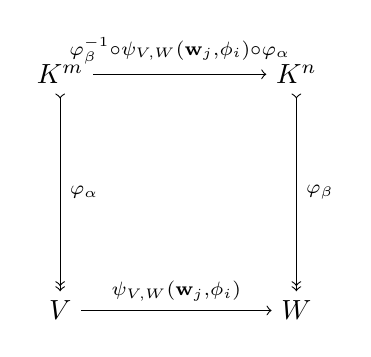
\begin{tikzpicture}[auto]
    \node (a) at (0, 3) {$K^m $};
    \node (b) at (0, 0) {$V$};
    \node (c) at (3, 3) {$K^n $};
    \node (d) at (3, 0) {$W$};
    \draw [->] (a) to node {$\scriptstyle \varphi_{\beta }^{-1} \circ \psi_{V,W} \left( {\bf w}_j ,\phi_i \right) \circ \varphi_{\alpha } $} (c);
    \draw [>->>] (a) to node {$\scriptstyle \varphi_{\alpha } $} (b);
    \draw [>->>] (c) to node {$\scriptstyle \varphi_{\beta } $} (d);
    \draw [->] (b) to node {$\scriptstyle \psi_{V,W} \left( {\bf w}_j ,\phi_i \right) $} (d);
  \end{tikzpicture} 
\end{center}
次のようになることから、
\begin{align*}
\varphi_{\beta}^{- 1} \circ \psi_{V,W}\left( \mathbf{w}_{j},\phi_{i} \right) \circ \varphi_{\alpha}\left( \mathbf{e}_{k} \right) &= \varphi_{\beta}^{- 1}\left( \psi_{V,W}\left( \mathbf{w}_{j},\phi_{i} \right)\left( \varphi_{\alpha}\left( \mathbf{e}_{k} \right) \right) \right)\\
&= \varphi_{\beta}^{- 1}\left( \psi_{V,W}\left( \mathbf{w}_{j},\phi_{i} \right)\left( \mathbf{v}_{k} \right) \right)\\
&= \varphi_{\beta}^{- 1}\left( \phi_{i}\left( \mathbf{v}_{k} \right)\mathbf{w}_{j} \right) = \varphi_{\beta}^{- 1}\left( \delta_{ik}\mathbf{w}_{j} \right)\\
&= \delta_{ik}\varphi_{\beta}^{- 1}\left( \mathbf{w}_{j} \right) = \delta_{ik}\mathbf{e}_{j} = \left( \delta_{ik}\delta_{jl} \right)_{l \in \varLambda_{n}}
\end{align*}
$\left[ \psi_{V,W}\left( \mathbf{w}_{j},\phi_{i} \right) \right]^{\beta}_{\alpha} = \left( \delta_{ik}\delta_{jl} \right)_{(k,l) \in \varLambda_{m} \times \varLambda_{n}}$が成り立つ。そこで、定理\ref{2.1.5.14}よりその表現行列$\left[ \psi_{V,W}\left( \mathbf{w}_{j},\phi_{i} \right) \right]^{\beta}_{\alpha}$を用いて次式のように定義される写像$F$はvector空間$L(V,W)$からvector空間$M_{nm}(K)$への線形同型写像であるので、
\begin{align*}
F:L(V,W)\overset{\sim}{\rightarrow}M_{nm}(K);\psi_{V,W}\left( \mathbf{w}_{j},\phi_{i} \right) \mapsto \left[ \psi_{V,W}\left( \mathbf{w}_{j},\phi_{i} \right) \right]_{\alpha}^{\beta}
\end{align*}
その行列$\left( \delta_{ik}\delta_{jl} \right)_{(k,l) \in \varLambda_{m} \times \varLambda_{n}}$はそのvector空間$M_{mn}(K)$の基底であることに注意すれば、定理\ref{2.1.5.2}よりその組$\left( \psi_{V,W}\left( \mathbf{w}_{j},\phi_{i} \right)\right)_{(i,j) \in \varLambda_{m} \times \varLambda_{n}}$はそのvector空間$L(V,W)$の基底をなす。\par
あとは定理\ref{2.4.5.2}より次のことが成り立つ。
\begin{itemize}
\item
  そのvector空間$W$の有限集合である族$\left\{ \mathbf{w}_{i} \right\}_{i \in \varLambda_{r}}$が与えられたとする。それらのvectors$\mathbf{w}_{i}$が線形独立であるなら、そのvector空間$V^{*}$の有限集合である任意の族$\left\{ f_{i} \right\}_{i \in \varLambda_{r}}$に対し、$\sum_{i \in \varLambda_{r}} {\psi_{V,W}\left( \mathbf{w}_{i},f_{i} \right)} = 0$が成り立つなら、$\forall i \in \varLambda_{r}$に対し、$f_{i} = 0$が成り立つ。
\item
  そのvector空間$V^{*}$の有限集合である族$\left\{ f_{i} \right\}_{i \in \varLambda_{r}}$が与えられたとする。それらのvectors$f_{i}$が線形独立であるなら、そのvector空間$W$の有限集合である任意の族$\left\{ \mathbf{w}_{i} \right\}_{i \in \varLambda_{r}}$に対し、$\sum_{i \in \varLambda_{r}} {\psi_{V,W}\left( \mathbf{w}_{i},f_{i} \right)} = 0$が成り立つなら、$\forall i \in \varLambda_{r}$に対し、$f_{i} = 0$が成り立つ。
\item
  そのvector空間$L(V,W)$は$\mathbf{w} \in W$、$f \in V^{*}$なるvector$\psi_{V,W}\left( \mathbf{w},f \right)$によって生成される。
\end{itemize}
これにより、そのvector空間$L(V,W)$とそのvector空間$W$のvectorのその双対空間$V^{*}$の線形形式の像倍へ写す双線形写像$\psi_{V,W}$との組$\left( L(V,W),\psi_{V,W} \right)$はそれらのvector空間たち$W$、$V^{*}$のtensor積である。\par
このとき、定理\ref{2.4.5.3}、定理\ref{2.4.5.4}よりある線形同型写像$\rho:W \otimes V^{*}\overset{\sim}{\rightarrow}L(V,W)$が存在して、$\psi_{V,W} = \rho \circ \otimes$が成り立ち、その線形写像$\rho$は$\rho\left( \mathbf{w} \otimes f \right):V \rightarrow W;\mathbf{v} \mapsto f\left( \mathbf{v} \right)\mathbf{w}$を満たす。したがって、$L(V,W) \cong W \otimes V^{*}$が成り立つ。
\end{proof}
\begin{thm}\label{2.4.5.8}
体$K$上の$m$次元vector空間$U$、$n$次元vector空間$V$、$o$次元vector空間$W$が与えられたとき、次のことが成り立つ。
\begin{itemize}
\item
  そのvector空間$W$のvectorのその双対空間$V^{*}$の線形形式の像倍へ写す双線形写像$\psi_{V,W}$について、$\forall\mathbf{w} \in W\forall f \in V^{*}$に対し、再双対空間$W^{**}$での自然な線形同型写像$\varphi$を用いて$\varphi\left( \mathbf{w} \right) = \widetilde{\mathbf{w}}$とおくと、$\psi_{V,W}^{*}\left( \mathbf{w},f \right) = \psi_{V,W}\left( f,\widetilde{\mathbf{w}} \right)$が成り立つ。
\item
  そのvector空間$V$のvectorのその双対空間$U^{*}$の線形形式の像倍へ写す双線形写像$\psi_{U,V}$、そのvector空間$W$のvectorのその双対空間$V^{*}$の線形形式の像倍へ写す双線形写像$\psi_{V,W}$が与えられたとき、$\forall\mathbf{v} \in V\forall\mathbf{w} \in W\forall f \in U^{*}\forall g \in V^{*}$に対し、$\psi_{V,W}\left( \mathbf{w},g \right) \circ \psi_{U,V}\left( \mathbf{v},f \right) = g\left( \mathbf{v} \right)\psi_{U,W}\left( \mathbf{w},f \right)$が成り立つ。
\item
  そのvector空間$V$のvectorのその双対空間$V^{*}$の線形形式の像倍へ写す双線形写像$\psi_{V,V}$について、そのvector空間の基底$\alpha$がどのように与えられても、$\forall\mathbf{v} \in V\forall f \in V^{*}$に対し、$\mathrm{tr}\left[ \psi_{V,V}\left( \mathbf{v},f \right) \right]_{\alpha}^{\alpha} = f\left( \mathbf{v} \right)$が成り立つ。
\end{itemize}
\end{thm}
\begin{proof}
体$K$上の$m$次元vector空間$U$、$n$次元vector空間$V$、$o$次元vector空間$W$が与えられたとき、そのvector空間$W$のvectorのその双対空間$V^{*}$の線形形式の像倍へ写す双線形写像$\psi_{V,W}$について、$\forall\mathbf{w} \in W\forall f \in V^{*}$に対し、再双対空間$W^{**}$での自然な線形同型写像$\varphi$を用いて$\varphi\left( \mathbf{w} \right) = \widetilde{\mathbf{w}}$とおくと、$\forall\mathbf{v} \in V\forall g \in W^{*}$に対し、次のようになる。
\begin{align*}
\psi_{V,W}^{*}\left( \mathbf{w},f \right)(g)\left( \mathbf{v} \right) &= g \circ \psi_{V,W}\left( \mathbf{w},f \right)\left( \mathbf{v} \right)\\
&= g\left( \psi_{V,W}\left( \mathbf{w},f \right)\left( \mathbf{v} \right) \right)\\
&= g\left( f\left( \mathbf{v} \right)\mathbf{w} \right)\\
&= f\left( \mathbf{v} \right)g\left( \mathbf{w} \right)\\
&= \widetilde{\mathbf{w}}(g)f\left( \mathbf{v} \right)\\
&= \left( \widetilde{\mathbf{w}}(g)f \right)\left( \mathbf{v} \right)\\
&= \psi_{V,W}\left( f,\widetilde{\mathbf{w}} \right)(g)\left( \mathbf{v} \right)
\end{align*}
以上より、$\psi_{V,W}^{*}\left( \mathbf{w},f \right) = \psi_{V,W}\left( f,\widetilde{\mathbf{w}} \right)$が成り立つ。\par
そのvector空間$V$のvectorのその双対空間$U^{*}$の線形形式の像倍へ写す双線形写像$\psi_{U,V}$、そのvector空間$W$のvectorのその双対空間$V^{*}$の線形形式の像倍へ写す双線形写像$\psi_{V,W}$が与えられたとき、$\forall\mathbf{v} \in V\forall\mathbf{w} \in W\forall f \in U^{*}\forall g \in V^{*}$に対し、その合成写像$\psi_{V,W}\left( \mathbf{w},g \right) \circ \psi_{U,V}\left( \mathbf{v},f \right)$が定義されて、$\forall\mathbf{u} \in U$に対し、次のようになる。
\begin{align*}
\psi_{V,W}\left( \mathbf{w},g \right) \circ \psi_{U,V}\left( \mathbf{v},f \right)\left( \mathbf{u} \right) &= \psi_{V,W}\left( \mathbf{w},g \right)\left( \psi_{U,V}\left( \mathbf{v},f \right)\left( \mathbf{u} \right) \right)\\
&= \psi_{V,W}\left( \mathbf{w},g \right)\left( f\left( \mathbf{u} \right)\mathbf{v} \right)\\
&= g\left( f\left( \mathbf{u} \right)\mathbf{v} \right)\mathbf{w}\\
&= f\left( \mathbf{u} \right)g\left( \mathbf{v} \right)\mathbf{w}\\
&= g\left( \mathbf{v} \right)\left( f\left( \mathbf{u} \right)\mathbf{w} \right)\\
&= g\left( \mathbf{v} \right)\psi_{U,W}\left( \mathbf{w},f \right)\left( \mathbf{u} \right)
\end{align*}
よって、$\psi_{V,W}\left( \mathbf{w},g \right) \circ \psi_{U,V}\left( \mathbf{v},f \right) = g\left( \mathbf{v} \right)\psi_{U,W}\left( \mathbf{w},f \right)$が得られる。\par
そのvector空間$V$のvectorのその双対空間$V^{*}$の線形形式の像倍へ写す双線形写像$\psi_{V,V}$について、そのvector空間の基底が$\alpha$と与えられたらば、$\forall\mathbf{v} \in V\forall f \in V^{*}$に対し、その基底$\alpha$に関する基底変換における線形同型写像$\varphi_{\alpha}$を用いて次式が成り立つので、
\begin{center}
  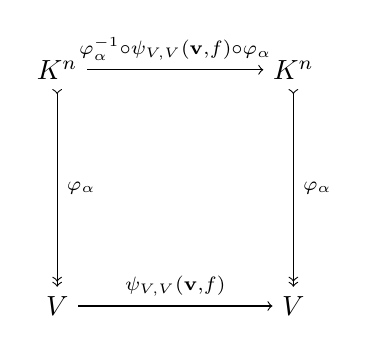
\begin{tikzpicture}[auto]
    \node (a) at (0, 3) {$K^n $};
    \node (b) at (0, 0) {$V$};
    \node (c) at (3, 3) {$K^n $};
    \node (d) at (3, 0) {$V$};
    \draw [->] (a) to node {$\scriptstyle \varphi_{\alpha }^{-1} \circ \psi_{V,V} \left( {\bf v} ,f \right) \circ \varphi_{\alpha } $} (c);
    \draw [>->>] (a) to node {$\scriptstyle \varphi_{\alpha } $} (b);
    \draw [>->>] (c) to node {$\scriptstyle \varphi_{\alpha } $} (d);
    \draw [->] (b) to node {$\scriptstyle \psi_{V,V} \left( {\bf v} ,f \right) $} (d);
  \end{tikzpicture} 
\end{center}
そのvector空間$K^{n}$の標準直交基底$\left\langle \mathbf{e}_{i} \right\rangle_{i \in \varLambda_{n}}$を用いて次式のようにおかれると、
\begin{align*}
\alpha = \left\langle \mathbf{v}_{i} \right\rangle_{i \in \varLambda_{n}},\ \ \mathbf{v} = \sum_{i \in \varLambda_{n}} {k_{i}\mathbf{v}_{i}}
\end{align*}
$\forall i \in \varLambda_{n}$に対し、次のようになる。
\begin{align*}
\varphi_{\alpha}^{- 1} \circ \psi_{V,V}\left( \mathbf{v},f \right) \circ \varphi_{\alpha}\left( \mathbf{e}_{i} \right) &= \varphi_{\alpha}^{- 1}\left( \psi_{V,V}\left( \mathbf{v},f \right)\left( \varphi_{\alpha}\left( \mathbf{e}_{i} \right) \right) \right)\\
&= \varphi_{\alpha}^{- 1}\left( \psi_{V,V}\left( \mathbf{v},f \right)\left( \mathbf{v}_{i} \right) \right)\\
&= \varphi_{\alpha}^{- 1}\left( f\left( \mathbf{v}_{i} \right)\mathbf{v} \right)\\
&= f\left( \mathbf{v}_{i} \right)\varphi_{\alpha}^{- 1}\left( \mathbf{v} \right)\\
&= f\left( \mathbf{v}_{i} \right)\varphi_{\alpha}^{- 1}\left( \sum_{j \in \varLambda_{n}} {k_{j}\mathbf{v}_{j}} \right)\\
&= \sum_{j \in \varLambda_{n}} {k_{j}f\left( \mathbf{v}_{i} \right)\varphi_{\alpha}^{- 1}\left( \mathbf{v}_{j} \right)}\\
&= \sum_{j \in \varLambda_{n}} {k_{j}f\left( \mathbf{v}_{i} \right)\mathbf{e}_{j}} = \begin{pmatrix}
k_{1}f\left( \mathbf{v}_{i} \right) \\
k_{2}f\left( \mathbf{v}_{i} \right) \\
 \vdots \\
k_{n}f\left( \mathbf{v}_{i} \right) \\
\end{pmatrix}
\end{align*}
以上より、その線形同型写像$\psi_{V,V}\left( \mathbf{v},f \right)$のその基底$\alpha$に関する表現行列$\left[ \psi_{V,V}\left( \mathbf{v},f \right) \right]_{\alpha}^{\alpha}$は、次のようになることから、
\begin{align*}
\left[ \psi_{V,V}\left( \mathbf{v},f \right) \right]_{\alpha}^{\alpha} = \begin{pmatrix}
k_{1}f\left( \mathbf{v}_{1} \right) & k_{1}f\left( \mathbf{v}_{2} \right) & \cdots & k_{1}f\left( \mathbf{v}_{n} \right) \\
k_{2}f\left( \mathbf{v}_{1} \right) & k_{2}f\left( \mathbf{v}_{2} \right) & \cdots & k_{2}f\left( \mathbf{v}_{n} \right) \\
 \vdots & \vdots & \ddots & \vdots \\
k_{n}f\left( \mathbf{v}_{1} \right) & k_{n}f\left( \mathbf{v}_{2} \right) & \cdots & k_{n}f\left( \mathbf{v}_{n} \right) \\
\end{pmatrix}
\end{align*}
次のようになる。
\begin{align*}
\mathrm{tr}\left[ \psi_{V,V}\left( \mathbf{v},f \right) \right]_{\alpha}^{\alpha} = \sum_{i \in \varLambda_{n}} {k_{i}f\left( \mathbf{v}_{i} \right)} = f\left( \sum_{i \in \varLambda_{n}} {k_{i}\mathbf{v}_{i}} \right) = f\left( \mathbf{v} \right)
\end{align*}
\end{proof}
%\hypertarget{ux7ddaux5f62ux5199ux50cfux306etensorux7a4d}{%
\subsubsection{線形写像のtensor積}%\label{ux7ddaux5f62ux5199ux50cfux306etensorux7a4d}}
\begin{thm}\label{2.4.5.9}
体$K$上の$m$次元vector空間$T$、$n$次元vector空間$U$、$o$次元vector空間$V$、$p$次元vector空間$W$が与えられたとき、$\forall\varphi \in L(T,V)\forall\chi \in L(U,W)$に対し、次式のような写像$\varPhi(\varphi,\chi)$は双線形写像である。
\begin{align*}
\varPhi(\varphi,\chi):T \times U \rightarrow V \otimes W;\left( \mathbf{t},\mathbf{u} \right) \mapsto \varphi\left( \mathbf{t} \right) \otimes \chi\left( \mathbf{u} \right)
\end{align*}
\end{thm}
\begin{proof}
体$K$上の$m$次元vector空間$T$、$n$次元vector空間$U$、$o$次元vector空間$V$、$p$次元vector空間$W$が与えられたとき、$\forall\varphi \in L(T,V)\forall\chi \in L(U,W)$に対し、次式のような写像$\varPhi(\varphi,\chi)$について、
\begin{align*}
\varPhi(\varphi,\chi):T \times U \rightarrow V \otimes W;\left( \mathbf{t},\mathbf{u} \right) \mapsto \varphi\left( \mathbf{t} \right) \otimes \chi\left( \mathbf{u} \right)
\end{align*}
$\forall k,l \in K\forall\mathbf{t},\mathbf{v} \in T\forall\mathbf{u} \in U$に対し、次のようになる。
\begin{align*}
\varPhi(\varphi,\chi)\left( k\mathbf{t} + l\mathbf{v},\mathbf{u} \right) &= \varphi\left( k\mathbf{t} + l\mathbf{v} \right) \otimes \chi\left( \mathbf{u} \right)\\
&= \left( k\varphi\left( \mathbf{t} \right) + l\varphi\left( \mathbf{v} \right) \right) \otimes \chi\left( \mathbf{u} \right)\\
&= k\varphi\left( \mathbf{t} \right) \otimes \chi\left( \mathbf{u} \right) + l\varphi\left( \mathbf{v} \right) \otimes \chi\left( \mathbf{u} \right)\\
&= k\varPhi(\varphi,\chi)\left( \mathbf{t},\mathbf{u} \right) + l\varPhi(\varphi,\chi)\left( \mathbf{v},\mathbf{u} \right)
\end{align*}
同様に、$\forall k,l \in K\forall\mathbf{t} \in T\forall\mathbf{u},\mathbf{v} \in U$に対し、次のようになる。
\begin{align*}
\varPhi(\varphi,\chi)\left( \mathbf{t},k\mathbf{u} + l\mathbf{v} \right) &= \varphi\left( \mathbf{t} \right) \otimes \chi\left( k\mathbf{u} + l\mathbf{v} \right)\\
&= \varphi\left( \mathbf{t} \right) \otimes \left( k\chi\left( \mathbf{u} \right) + l\chi\left( \mathbf{v} \right) \right)\\
&= k\varphi\left( \mathbf{t} \right) \otimes \chi\left( \mathbf{u} \right) + l\varphi\left( \mathbf{t} \right) \otimes \chi\left( \mathbf{v} \right)\\
&= k\varPhi(\varphi,\chi)\left( \mathbf{t},\mathbf{u} \right) + l\varPhi(\varphi,\chi)\left( \mathbf{t},\mathbf{v} \right)
\end{align*}
よって、$\forall\varphi \in L(T,V)\forall\chi \in L(U,W)$に対し、その写像$\varPhi(\varphi,\chi)$は双線形写像である。
\end{proof}
\begin{thm}\label{2.4.5.10}
体$K$上の$m$次元vector空間$T$、$n$次元vector空間$U$、$o$次元vector空間$V$、$p$次元vector空間$W$が与えられたとき、$\forall\varphi \in L(T,V)\forall\chi \in L(U,W)$に対し、次式のような双線形写像$\varPhi(\varphi,\chi)$について、
\begin{align*}
\varPhi(\varphi,\chi):T \times U \rightarrow V \otimes W;\left( \mathbf{t},\mathbf{u} \right) \mapsto \varphi\left( \mathbf{t} \right) \otimes \chi\left( \mathbf{u} \right)
\end{align*}
ある線形写像$\rho(\varphi,\chi):T \otimes U \rightarrow V \otimes W$が一意的に存在して、$\forall\left( \mathbf{t},\mathbf{u} \right) \in T \times U$に対し、次式が成り立つ。
\begin{align*}
\rho(\varphi,\chi)\left( \mathbf{t} \otimes \mathbf{u} \right) = \varphi\left( \mathbf{t} \right) \otimes \chi\left( \mathbf{u} \right)
\end{align*}
\end{thm}
\begin{proof}
体$K$上の$m$次元vector空間$T$、$n$次元vector空間$U$、$o$次元vector空間$V$、$p$次元vector空間$W$が与えられたとき、$\forall\varphi \in L(T,V)\forall\chi \in L(U,W)$に対し、次式のような双線形写像$\varPhi(\varphi,\chi)$について、
\begin{align*}
\varPhi(\varphi,\chi):T \times U \rightarrow V \otimes W;\left( \mathbf{t},\mathbf{u} \right) \mapsto \varphi\left( \mathbf{t} \right) \otimes \chi\left( \mathbf{u} \right)
\end{align*}
$\forall\left( \mathbf{t},\mathbf{u} \right) \in T \times U$に対し、$\rho(\varphi,\chi)\left( \mathbf{t} \otimes \mathbf{u} \right) = \varphi\left( \mathbf{t} \right) \otimes \chi\left( \mathbf{u} \right)$なる線形写像$\rho(\varphi,\chi):T \otimes U \rightarrow V \otimes W$が考えられそれらのvector空間たち$T$、$U$の基底たち$\left\langle \mathbf{t}_{i} \right\rangle_{i \in \varLambda_{m}}$、$\left\langle \mathbf{u}_{j} \right\rangle_{j \in \varLambda_{n}}$を用いて、$\forall(i,j) \in \varLambda_{m} \times \varLambda_{n}$に対し、次式のようにおかれれば、
\begin{align*}
\mathbf{t} = \sum_{i \in \varLambda_{m}} {t_{i}\mathbf{t}_{i}},\ \ \mathbf{u} = \sum_{j \in \varLambda_{n}} {u_{j}\mathbf{u}_{j}}
\end{align*}
次のようになることから、
\begin{align*}
\varPhi(\varphi,\chi)\left( \mathbf{t},\mathbf{u} \right) &= \varphi\left( \mathbf{t} \right) \otimes \chi\left( \mathbf{u} \right)\\
&= \varphi\left( \sum_{i \in \varLambda_{m}} {t_{i}\mathbf{t}_{i}} \right) \otimes \chi\left( \sum_{j \in \varLambda_{n}} {u_{j}\mathbf{u}_{j}} \right)\\
&= \sum_{j \in \varLambda_{n}} {t_{i}\varphi\left( \mathbf{t}_{i} \right)} \otimes \sum_{j \in \varLambda_{n}} {u_{j}\chi\left( \mathbf{u}_{j} \right)}\\
&= \sum_{i \in \varLambda_{m}} {\sum_{j \in \varLambda_{n}} {t_{i}u_{j}\varphi\left( \mathbf{t}_{i} \right) \otimes \chi\left( \mathbf{u}_{j} \right)}}\\
&= \sum_{i \in \varLambda_{m}} {\sum_{j \in \varLambda_{n}} {t_{i}u_{j}\rho(\varphi,\chi)\left( \mathbf{t}_{i} \otimes \mathbf{u}_{j} \right)}}\\
&= \rho(\varphi,\chi)\left( \sum_{i \in \varLambda_{m}} {\sum_{j \in \varLambda_{n}} {t_{i}u_{j}\mathbf{t}_{i} \otimes \mathbf{u}_{j}}} \right)\\
&= \rho(\varphi,\chi)\left( \sum_{i \in \varLambda_{m}} {t_{i}\mathbf{t}_{i}} \otimes \sum_{j \in \varLambda_{n}} {u_{j}\mathbf{u}_{j}} \right)\\
&= \rho(\varphi,\chi)\left( \mathbf{t} \otimes \mathbf{u} \right) = \rho(\varphi,\chi) \circ \otimes \left( \mathbf{t},\mathbf{u} \right)
\end{align*}
定理\ref{2.4.5.3}よりある線形写像$\rho(\varphi,\chi):T \otimes U \rightarrow V \otimes W$が一意的に存在して、$\varPhi(\varphi,\chi) = \rho(\varphi,\chi) \circ \otimes$が成り立つ。
\end{proof}
\begin{thm}\label{2.4.5.11}
体$K$上の$m$次元vector空間$T$、$n$次元vector空間$U$、$o$次元vector空間$V$、$p$次元vector空間$W$が与えられたとき、$\forall\varphi \in L(T,V)\forall\chi \in L(U,W)\forall\left( \mathbf{t},\mathbf{u} \right) \in T \times U$に対し、$\rho(\varphi,\chi)\left( \mathbf{t} \otimes \mathbf{u} \right) = \varphi\left( \mathbf{t} \right) \otimes \chi\left( \mathbf{u} \right)$なる線形写像$\rho(\varphi,\chi):T \otimes U \rightarrow V \otimes W$を用いた次式のような写像$\rho$は双線形写像である。
\begin{align*}
\rho:L(T,V) \times L(U,W) \rightarrow L(T \otimes U,V \otimes W);(\varphi,\chi) \mapsto \rho(\varphi,\chi)
\end{align*}
\end{thm}
\begin{proof}
体$K$上の$m$次元vector空間$T$、$n$次元vector空間$U$、$o$次元vector空間$V$、$p$次元vector空間$W$が与えられたとき、$\forall\varphi \in L(T,V)\forall\chi \in L(U,W)\forall\left( \mathbf{t},\mathbf{u} \right) \in T \times U$に対し、$\rho(\varphi,\chi)\left( \mathbf{t} \otimes \mathbf{u} \right) = \varphi\left( \mathbf{t} \right) \otimes \chi\left( \mathbf{u} \right)$なる線形写像$\rho(\varphi,\chi):T \otimes U \rightarrow V \otimes W$を用いた次式のような写像$\rho$について、
\begin{align*}
\rho:L(T,V) \times L(U,W) \rightarrow L(T \otimes U,V \otimes W);(\varphi,\chi) \mapsto \rho(\varphi,\chi)
\end{align*}
$\forall k,l \in K\forall\varphi,\psi \in L(T,V)\forall\chi \in L(U,W)$に対し、線形写像$\rho(k\varphi + l\psi,\chi)$が定義されて、$\forall\mathbf{T} \in T \otimes U$に対し、それらのvector空間たち$T$、$U$の基底たち$\left\langle \mathbf{t}_{i} \right\rangle_{i \in \varLambda_{m}}$、$\left\langle \mathbf{u}_{j} \right\rangle_{j \in \varLambda_{n}}$を用いて定理\ref{2.4.5.2}より$\mathbf{T} = \sum_{(i,j) \in \varLambda_{m} \times \varLambda_{n}} {\xi_{ij}\mathbf{t}_{i} \otimes \mathbf{u}_{j}} \in T \otimes U$とおかれると、次のようになるかつ、
\begin{align*}
\rho(k\varphi + l\psi,\chi)\left( \mathbf{T} \right) &= \rho(k\varphi + l\psi,\chi)\left( \sum_{(i,j) \in \varLambda_{m} \times \varLambda_{n}} {\xi_{ij}\mathbf{t}_{i} \otimes \mathbf{u}_{j}} \right)\\
&= \sum_{(i,j) \in \varLambda_{m} \times \varLambda_{n}} {\xi_{ij}\rho(k\varphi + l\psi,\chi)\left( \mathbf{t}_{i} \otimes \mathbf{u}_{j} \right)}\\
&= \sum_{(i,j) \in \varLambda_{m} \times \varLambda_{n}} {\xi_{ij}(k\varphi + l\psi)\left( \mathbf{t}_{i} \right) \otimes \chi\left( \mathbf{u}_{j} \right)}\\
&= \sum_{(i,j) \in \varLambda_{m} \times \varLambda_{n}} {\xi_{ij}\left( k\varphi\left( \mathbf{t}_{i} \right) + l\psi\left( \mathbf{t}_{i} \right) \right) \otimes \chi\left( \mathbf{u}_{j} \right)}\\
&= \sum_{(i,j) \in \varLambda_{m} \times \varLambda_{n}} {\xi_{ij}\left( k\varphi\left( \mathbf{t}_{i} \right) \otimes \chi\left( \mathbf{u}_{j} \right) + l\psi\left( \mathbf{t}_{i} \right) \otimes \chi\left( \mathbf{u}_{j} \right) \right)}\\
&= k\sum_{(i,j) \in \varLambda_{m} \times \varLambda_{n}} {\xi_{ij}\varphi\left( \mathbf{t}_{i} \right) \otimes \chi\left( \mathbf{u}_{j} \right)} + l\sum_{(i,j) \in \varLambda_{m} \times \varLambda_{n}} {\xi_{ij}\psi\left( \mathbf{t}_{i} \right) \otimes \chi\left( \mathbf{u}_{j} \right)}\\
&= k\sum_{(i,j) \in \varLambda_{m} \times \varLambda_{n}} {\xi_{ij}\rho(\varphi,\chi)\left( \mathbf{t}_{i} \otimes \mathbf{u}_{j} \right)} + l\sum_{(i,j) \in \varLambda_{m} \times \varLambda_{n}} {\xi_{ij}\rho(\psi,\chi)\left( \mathbf{t}_{i} \otimes \mathbf{u}_{j} \right)}\\
&= k\rho(\varphi,\chi)\left( \sum_{(i,j) \in \varLambda_{m} \times \varLambda_{n}} {\xi_{ij}\mathbf{t}_{i} \otimes \mathbf{u}_{j}} \right) + l\rho(\psi,\chi)\left( \sum_{(i,j) \in \varLambda_{m} \times \varLambda_{n}} {\xi_{ij}\mathbf{t}_{i} \otimes \mathbf{u}_{j}} \right)\\
&= k\rho(\varphi,\chi)\left( \mathbf{T} \right) + l\rho(\psi,\chi)\left( \mathbf{T} \right)\\
&= \left( k\rho(\varphi,\chi) + l\rho(\psi,\chi) \right)\left( \mathbf{T} \right)
\end{align*}
$\forall k,l \in K\forall\varphi \in L(T,V)\forall\chi,\psi \in L(U,W)$に対し、線形写像$\rho(\varphi,k\chi + l\psi)$が定義されて、$\forall\mathbf{T} \in T \otimes U$に対し、定理\ref{2.4.5.2}より$\mathbf{T} = \sum_{(i,j) \in \varLambda_{m} \times \varLambda_{n}} {\xi_{ij}\mathbf{t}_{i} \otimes \mathbf{u}_{j}} \in T \otimes U$とおかれると、次のようになるので、
\begin{align*}
\rho(\varphi,k\chi + l\psi)\left( \mathbf{T} \right) &= \rho(\varphi,k\chi + l\psi)\left( \sum_{(i,j) \in \varLambda_{m} \times \varLambda_{n}} {\xi_{ij}\mathbf{t}_{i} \otimes \mathbf{u}_{j}} \right)\\
&= \sum_{(i,j) \in \varLambda_{m} \times \varLambda_{n}} {\xi_{ij}\rho(\varphi,k\chi + l\psi)\left( \mathbf{t}_{i} \otimes \mathbf{u}_{j} \right)}\\
&= \sum_{(i,j) \in \varLambda_{m} \times \varLambda_{n}} {\xi_{ij}\varphi\left( \mathbf{t}_{i} \right) \otimes (k\chi + l\psi)\left( \mathbf{u}_{j} \right)}\\
&= \sum_{(i,j) \in \varLambda_{m} \times \varLambda_{n}} {\xi_{ij}\varphi\left( \mathbf{t}_{i} \right) \otimes \left( k\chi\left( \mathbf{u}_{j} \right) + l\psi\left( \mathbf{u}_{j} \right) \right)}\\
&= \sum_{(i,j) \in \varLambda_{m} \times \varLambda_{n}} {\xi_{ij}\left( k\varphi\left( \mathbf{t}_{i} \right) \otimes \chi\left( \mathbf{u}_{j} \right) + l\varphi\left( \mathbf{t}_{i} \right) \otimes \psi\left( \mathbf{u}_{j} \right) \right)}\\
&= k\sum_{(i,j) \in \varLambda_{m} \times \varLambda_{n}} {\xi_{ij}\varphi\left( \mathbf{t}_{i} \right) \otimes \chi\left( \mathbf{u}_{j} \right)} + l\sum_{(i,j) \in \varLambda_{m} \times \varLambda_{n}} {\xi_{ij}\varphi\left( \mathbf{t}_{i} \right) \otimes \psi\left( \mathbf{u}_{j} \right)}\\
&= k\sum_{(i,j) \in \varLambda_{m} \times \varLambda_{n}} {\xi_{ij}\rho(\varphi,\chi)\left( \mathbf{t}_{i} \otimes \mathbf{u}_{j} \right)} + l\sum_{(i,j) \in \varLambda_{m} \times \varLambda_{n}} {\xi_{ij}\rho(\varphi,\psi)\left( \mathbf{t}_{i} \otimes \mathbf{u}_{j} \right)}\\
&= k\rho(\varphi,\chi)\left( \sum_{(i,j) \in \varLambda_{m} \times \varLambda_{n}} {\xi_{ij}\mathbf{t}_{i} \otimes \mathbf{u}_{j}} \right) + l\rho(\varphi,\psi)\left( \sum_{(i,j) \in \varLambda_{m} \times \varLambda_{n}} {\xi_{ij}\mathbf{t}_{i} \otimes \mathbf{u}_{j}} \right)\\
&= k\rho(\varphi,\chi)\left( \mathbf{T} \right) + l\rho(\varphi,\psi)\left( \mathbf{T} \right)\\
&= \left( k\rho(\varphi,\chi) + l\rho(\varphi,\psi) \right)\left( \mathbf{T} \right)
\end{align*}
その写像$\rho$は双線形写像である。
\end{proof}
\begin{thm}\label{2.4.5.12}
体$K$上の$m$次元vector空間$T$、$n$次元vector空間$U$、$o$次元vector空間$V$、$p$次元vector空間$W$が与えられたとき、vector空間$L(T \otimes U,V \otimes W)$を用いた、$\forall\varphi \in L(T,V)\forall\chi \in L(U,W)\forall\left( \mathbf{t},\mathbf{u} \right) \in T \times U$に対し、$\rho(\varphi,\chi)\left( \mathbf{t} \otimes \mathbf{u} \right) = \varphi\left( \mathbf{t} \right) \otimes \chi\left( \mathbf{u} \right)$なる線形写像$\rho(\varphi,\chi):T \otimes U \rightarrow V \otimes W$を用いた次式のような写像$\rho$との組$\left( L(T \otimes U,V \otimes W),\rho \right)$はtensor積である。
\begin{align*}
\rho:L(T,V) \times L(U,W) \rightarrow L(T \otimes U,V \otimes W);(\varphi,\chi) \mapsto \rho(\varphi,\chi)
\end{align*}
\end{thm}
\begin{proof}
体$K$上の$m$次元vector空間$T$、$n$次元vector空間$U$、$o$次元vector空間$V$、$p$次元vector空間$W$が与えられたとき、vector空間$L(T \otimes U,V \otimes W)$を用いた、$\forall\varphi \in L(T,V)\forall\chi \in L(U,W)\forall\left( \mathbf{t},\mathbf{u} \right) \in T \times U$に対し、$\rho(\varphi,\chi)\left( \mathbf{t} \otimes \mathbf{u} \right) = \varphi\left( \mathbf{t} \right) \otimes \chi\left( \mathbf{u} \right)$なる線形写像$\rho(\varphi,\chi):T \otimes U \rightarrow V \otimes W$を用いた次式のような写像$\rho$との組$\left( L(T \otimes U,V \otimes W),\rho \right)$について、その写像$\rho$が双線形写像となるのはすでに定理\ref{2.4.5.11}でみた。\par
そこで、それらのvector空間たち$T$、$U$、$V$、$W$の基底たち$\left\langle \mathbf{t}_{i} \right\rangle_{i \in \varLambda_{m}}$、$\left\langle \mathbf{u}_{j} \right\rangle_{j \in \varLambda_{n}}$、$\left\langle \mathbf{v}_{i} \right\rangle_{i \in \varLambda_{o}}$、$\left\langle \mathbf{w}_{j} \right\rangle_{j \in \varLambda_{p}}$を用いれば、定理\ref{2.4.5.2}よりそれらの組々$\left\langle \mathbf{t}_{i} \otimes \mathbf{u}_{j} \right\rangle_{(i,j) \in \varLambda_{m} \times \varLambda_{n}}$、$\left\langle \mathbf{v}_{i} \otimes \mathbf{w}_{j} \right\rangle_{(i,j) \in \varLambda_{o} \times \varLambda_{p}}$はそれぞれそれらのvector空間たち$T \otimes U$、$V \otimes W$の基底となるので、$\forall e \in \varLambda_{m}\forall(i,j) \in \varLambda_{m} \times \varLambda_{o}$に対し、$\varphi_{ij}\left( \mathbf{t}_{e} \right) = \delta_{ie}\mathbf{v}_{j}$となる線形写像たち$\varphi_{ij}:T \rightarrow V$、$\forall g \in \varLambda_{n}\forall(k,l) \in \varLambda_{n} \times \varLambda_{p}$に対し、$\chi_{kl}\left( \mathbf{u}_{g} \right) = \delta_{kg}\mathbf{w}_{l}$となる線形写像たち$\chi_{kl}:U \rightarrow W$が考えられれば、$\left\langle \mathbf{t}_{i} \right\rangle_{i \in \varLambda_{m}} = \alpha$、$\left\langle \mathbf{u}_{j} \right\rangle_{j \in \varLambda_{n}} = \beta$、$\left\langle \mathbf{v}_{i} \right\rangle_{i \in \varLambda_{o}} = \gamma$、$\left\langle \mathbf{w}_{j} \right\rangle_{j \in \varLambda_{p}} = \delta$とおいて、vector空間たち$K^{m}$、$K^{n}$、$K^{o}$、$K^{p}$の標準直交基底たち$\left\langle \mathbf{d}_{e} \right\rangle_{e \in \varLambda_{m}}$、$\left\langle \mathbf{e}_{g} \right\rangle_{g \in \varLambda_{n}}$、$\left\langle \mathbf{f}_{f} \right\rangle_{f \in \varLambda_{o}}$、$\left\langle \mathbf{g}_{h} \right\rangle_{h \in \varLambda_{p}}$、それらの基底たち$\alpha$、$\beta$、$\gamma$、$\delta$の基底変換における線形同型写像たち$\varphi_{\alpha}$、$\varphi_{\beta}$、$\varphi_{\gamma}$、$\varphi_{\delta}$を用いて$\forall e \in \varLambda_{m}\forall g \in \varLambda_{n}$に対し、次のようになることから、
\begin{align*}
\varphi_{\gamma}^{- 1} \circ \varphi_{ij} \circ \varphi_{\alpha}\left( \mathbf{d}_{e} \right) &= \varphi_{\gamma}^{- 1}\left( \varphi_{ij}\left( \varphi_{\alpha}\left( \mathbf{d}_{e} \right) \right) \right)\\
&= \varphi_{\gamma}^{- 1}\left( \varphi_{ij}\left( \mathbf{t}_{e} \right) \right)\\
&= \varphi_{\gamma}^{- 1}\left( \delta_{ie}\mathbf{v}_{j} \right)\\
&= \delta_{ie}\varphi_{\gamma}^{- 1}\left( \mathbf{v}_{j} \right)\\
&= \delta_{ie}\mathbf{f}_{j}\\
&= \left( \delta_{ie}\delta_{jf} \right)_{f \in \varLambda_{o}}\\
\varphi_{\gamma}^{- 1} \circ \chi_{kl} \circ \varphi_{\alpha}\left( \mathbf{e}_{g} \right) &= \varphi_{\gamma}^{- 1}\left( \chi_{kl}\left( \varphi_{\alpha}\left( \mathbf{e}_{g} \right) \right) \right)\\
&= \varphi_{\gamma}^{- 1}\left( \chi_{kl}\left( \mathbf{u}_{g} \right) \right)\\
&= \varphi_{\gamma}^{- 1}\left( \delta_{kg}\mathbf{w}_{l} \right)\\
&= \delta_{kg}\varphi_{\gamma}^{- 1}\left( \mathbf{w}_{l} \right)\\
&= \delta_{kg}\mathbf{g}_{l}\\
&= \left( \delta_{kg}\delta_{lh} \right)_{h \in \varLambda_{p}}
\end{align*}
$\left[ \varphi_{ij} \right]^{\gamma}_{\alpha} = \left( \delta_{ie}\delta_{jf} \right)_{(e,f) \in \varLambda_{m} \times \varLambda_{o}}$、$\left[ \chi_{kl} \right]^{\delta}_{\beta} = \left( \delta_{kg}\delta_{lh} \right)_{(g,h) \in \varLambda_{n} \times \varLambda_{p}}$が成り立つ。そこで、これらの行列たちがそれぞれそれらのvector空間たち$M_{mo}(K)$、$M_{np}(K)$の基底たちであることに注意すれば、そのvector空間$T$からそのvector空間$V$への線形写像からそれらの基底たち$\alpha$、$\gamma$に関する表現行列へ写す写像、そのvector空間$U$からそのvector空間$W$への線形写像からそれらの基底たち$\beta$、$\delta$に関する表現行列へ写す写像がいづれも定理\ref{2.1.5.14}より線形同型写像となっているので、定理\ref{2.1.5.2}よりその組々$\left( \varphi_{ij} \right)_{(i,j) \in \varLambda_{m} \times \varLambda_{o}}$、$\left(\chi_{kl}\right)_{(k,l) \in \varLambda_{n} \times \varLambda_{p}}$はそれぞれvector空間たち$L(T,V)$、$L(U,W)$の基底をなす。\par
したがって、$\forall(i,j) \in \varLambda_{m} \times \varLambda_{o}\forall(k,l) \in \varLambda_{n} \times \varLambda_{p}\forall e \in \varLambda_{m}\forall g \in \varLambda_{n}$に対し、次のようになる。
\begin{align*}
\rho\left( \varphi_{ij},\chi_{kl} \right)\left( \mathbf{t}_{e} \otimes \mathbf{u}_{g} \right) &= \varphi_{ij}\left( \mathbf{t}_{e} \right) \otimes \chi_{kl}\left( \mathbf{u}_{g} \right)\\
&= \delta_{ie}\mathbf{v}_{j} \otimes \delta_{kg}\mathbf{w}_{l}\\
&= \delta_{ie}\delta_{kg}\mathbf{v}_{j} \otimes \mathbf{w}_{l}
\end{align*}
そこで、それらのvector空間たち$T \otimes U$、$V \otimes W$の基底たちそれぞれ$\alpha \otimes \beta$、$\gamma \otimes \delta$、これらの基底たち$\alpha \otimes \beta$、$\gamma \otimes \delta$に関する基底変換における線形同型写像たち$\varphi_{\alpha \otimes \beta}$、$\varphi_{\gamma \otimes \delta}$、それらのvector空間たち$K^{mn}$、$K^{op}$の標準直交基底たち$\left\langle \mathbf{d}_{eg} \right\rangle_{(e,g) \in \varLambda_{m} \times \varLambda_{n}}$、$\left\langle \mathbf{e}_{fh} \right\rangle_{(f,h) \in \varLambda_{o} \times \varLambda_{p}}$が用いられると、次のようになることから、
\begin{align*}
\varphi_{\gamma \otimes \delta}^{- 1} \circ \rho\left( \varphi_{ij},\chi_{kl} \right) \circ \varphi_{\alpha \otimes \beta}\left( \mathbf{d}_{eg} \right) &= \varphi_{\gamma \otimes \delta}^{- 1}\left( \rho\left( \varphi_{ij},\chi_{kl} \right)\left( \varphi_{\alpha \otimes \beta}\left( \mathbf{d}_{eg} \right) \right) \right)\\
&= \varphi_{\gamma \otimes \delta}^{- 1}\left( \rho\left( \varphi_{ij},\chi_{kl} \right)\left( \mathbf{t}_{e} \otimes \mathbf{u}_{g} \right) \right)\\
&= \varphi_{\gamma \otimes \delta}^{- 1}\left( \delta_{ie}\delta_{kg}\mathbf{v}_{j} \otimes \mathbf{w}_{l} \right)\\
&= \delta_{ie}\delta_{kg}\varphi_{\gamma \otimes \delta}^{- 1}\left( \mathbf{v}_{j} \otimes \mathbf{w}_{l} \right)\\
&= \delta_{ie}\delta_{kg}\mathbf{e}_{jl}\\
&= \left( \delta_{ie}\delta_{kg}\delta_{jf}\delta_{lh} \right)_{(f,h) \in \varLambda_{o} \times \varLambda_{p}}
\end{align*}
$\left[ \rho\left( \varphi_{ij},\chi_{kl} \right) \right]^{\gamma \otimes \delta}_{\alpha \otimes \beta} = \left( \delta_{ie}\delta_{kg}\delta_{jf}\delta_{lh} \right)_{(e,f,g,h) \in \varLambda_{m} \times \varLambda_{o} \times \varLambda_{n} \times \varLambda_{p}}$が成り立つ。そこで、これがそのvector空間$K^{m \times o \times n \times p}$の基底であることに注意すれば、そのvector空間$T \otimes U$からそのvector空間$V \otimes W$への線形写像からそれらの基底たち$\alpha \otimes \beta$、$\gamma \otimes \delta$に関する表現行列へ写す写像が定理\ref{2.1.5.14}より線形同型写像となっているので、定理\ref{2.1.5.2}よりその組$\left(\rho\left( \varphi_{ij},\chi_{kl} \right)\right)_{(i,j,k,l) \in \varLambda_{m} \times \varLambda_{o}\times \varLambda_{n} \times \varLambda_{p}}$はそのvector空間$L(T \otimes U,V \otimes W)$の基底をなす。\par
定理\ref{2.4.5.2}よりよって、その線形写像$\rho(\varphi,\chi):T \otimes U \rightarrow V \otimes W$を用いたその写像$\rho$との組$\left( L(T \otimes U,V \otimes W),\rho \right)$はtensor積である。
\end{proof}
\begin{thm}\label{2.4.5.13}
体$K$上の$m$次元vector空間$T$、$n$次元vector空間$U$、$o$次元vector空間$V$、$p$次元vector空間$W$が与えられたとき、次式が成り立つ。
\begin{align*}
L(T \otimes U,V \otimes W) \cong L(T,V) \otimes L(U,W)
\end{align*}
このとき、ある線形同型写像$\sigma:L(T,V) \otimes L(U,W)\overset{\sim}{\rightarrow}L(T \otimes U,V \otimes W)$が一意的に存在して、$\forall(\varphi,\chi) \in L(T,V) \times L(U,W)\forall\left( \mathbf{t},\mathbf{u} \right) \in T \times U$に対し、$\varphi\left( \mathbf{t} \right) \otimes \chi\left( \mathbf{u} \right) = \sigma(\varphi \otimes \chi)\left( \mathbf{t} \otimes \mathbf{u} \right)$が成り立つ。
\end{thm}
\begin{proof}
体$K$上の$m$次元vector空間$T$、$n$次元vector空間$U$、$o$次元vector空間$V$、$p$次元vector空間$W$が与えられたとき、定理\ref{2.4.5.12}よりvector空間$L(T \otimes U,V \otimes W)$を用いた、$\forall\varphi \in L(T,V)\forall\chi \in L(U,W)\forall\left( \mathbf{t},\mathbf{u} \right) \in T \times U$に対し、$\rho(\varphi,\chi)\left( \mathbf{t} \otimes \mathbf{u} \right) = \varphi\left( \mathbf{t} \right) \otimes \chi\left( \mathbf{u} \right)$なる線形写像$\rho(\varphi,\chi):T \otimes U \rightarrow V \otimes W$を用いた次式のような写像$\rho$との組$\left( L(T \otimes U,V \otimes W),\rho \right)$はtensor積である。そこで、定理\ref{2.4.5.4}より次式が成り立つ。
\begin{align*}
L(T \otimes U,V \otimes W) \cong L(T,V) \otimes L(U,W)
\end{align*}\par
また、定理\ref{2.4.5.3}、定理\ref{2.4.5.4}よりある線形同型写像$\sigma:L(T,V) \otimes L(U,W)\overset{\sim}{\rightarrow}L(T \otimes U,V \otimes W)$が一意的に存在して、$\rho = \sigma \circ \otimes$が成り立つので、$\forall(\varphi,\chi) \in L(T,V) \times L(U,W)\forall\left( \mathbf{t},\mathbf{u} \right) \in T \times U$に対し、次のようになる。
\begin{align*}
\varphi\left( \mathbf{t} \right) \otimes \chi\left( \mathbf{u} \right) &= \rho(\varphi,\chi)\left( \mathbf{t} \otimes \mathbf{u} \right)\\
&= \sigma \circ \otimes (\varphi,\chi)\left( \mathbf{t} \otimes \mathbf{u} \right)\\
&= \sigma(\varphi \otimes \chi)\left( \mathbf{t} \otimes \mathbf{u} \right)
\end{align*}
\end{proof}
%\hypertarget{tensorux7a4dux3068ux7ddaux5f62ux540cux578b}{%
\subsubsection{tensor積と線形同型}%\label{tensorux7a4dux3068ux7ddaux5f62ux540cux578b}}
\begin{thm}\label{2.4.5.14}
体$K$上の$m$次元vector空間$V$、$n$次元vector空間$W$が与えられたとき、次式が成り立つ。
\begin{align*}
(V \otimes W)^{*} \cong V^{*} \otimes W^{*}
\end{align*}
このとき、ある線形同型写像$\varSigma:V^{*} \otimes W^{*}\overset{\sim}{\rightarrow}(V \otimes W)^{*}$が存在して、$\forall(\varphi,\chi) \in V^{*} \times W^{*}\forall\left( \mathbf{v},\mathbf{w} \right) \in V \times W$に対し、$\varSigma(\varphi \otimes \chi)\left( \mathbf{v} \otimes \mathbf{w} \right) = \varphi\left( \mathbf{v} \right)\chi\left( \mathbf{w} \right)$が成り立つ。
\end{thm}
\begin{proof}
体$K$上の$m$次元vector空間$V$、$n$次元vector空間$W$が与えられたとき、定理\ref{2.4.5.13}より次式が成り立つ。
\begin{align*}
L(V \otimes W,K \otimes K) \cong L(V,K) \otimes L(W,K)
\end{align*}
そこで、$V^{*} = L(V,K)$、$W^{*} = L(W,K)$が成り立つことにより次式が成り立つ。
\begin{align*}
L(V \otimes W,K \otimes K) \cong V^{*} \otimes W^{*}
\end{align*}\par
ところで、組$(K, \cdot )$について、$\forall k,l \in K\forall\alpha,\beta,\gamma \in K$に対し、次のようになることから、
\begin{align*}
(k\alpha + l\gamma)\beta = k\alpha\beta + l\gamma\beta,\ \ \alpha(k\beta + l\gamma) = k\alpha\beta + l\alpha\gamma
\end{align*}
その写像$\cdot :K \times K \rightarrow K;(\alpha,\beta) \mapsto \alpha\beta$は双線形写像である。さらに、$\forall k \in K$に対し、$k \neq 0$のとき、$kl = lk = 0$が成り立つなら、$l = 0$が成り立つかつ、そのvector空間$K$はその双線形写像$\cdot$の値域と等しいので、その組$(K, \cdot )$はそれらのvector空間たち$K$のtensor積である。また、定理\ref{2.4.5.3}、定理\ref{2.4.5.4}より直ちにある線形同型写像$\sigma$が一意的に存在して、$\cdot = \sigma \circ \otimes$が成り立つ。\par
そこで、$\forall\mathbf{T} \in V \otimes W$に対し、$\dim{K \otimes K} = 1$に注意すれば、次のようになることから、
\begin{align*}
\sigma \circ f\left( \mathbf{T} \right) &= \sigma(k\alpha \otimes \beta)\\
&= k\sigma(\alpha \otimes \beta)\\
&= k\alpha\beta \in K
\end{align*}
次式のような写像$F$が考えられれば、
\begin{align*}
F:L(V \otimes W,K \otimes K) \rightarrow (V \otimes W)^{*};f \mapsto \sigma \circ f
\end{align*}
$\forall k,l \in K\forall f,g \in L(V \otimes W,K \otimes K)$に対し、$kf + lg \in L(V \otimes W,K \otimes K)$が成り立って、$\forall\mathbf{T} \in V \otimes W$に対し、次のようになる。
\begin{align*}
F(kf + lg)\left( \mathbf{T} \right) &= \sigma \circ (kf + lg)\left( \mathbf{T} \right)\\
&= \sigma\left( kf\left( \mathbf{T} \right) + lg\left( \mathbf{T} \right) \right)\\
&= k\sigma\left( f\left( \mathbf{T} \right) \right) + l\sigma\left( g\left( \mathbf{T} \right) \right)\\
&= k\sigma \circ f\left( \mathbf{T} \right) + l\sigma \circ g\left( \mathbf{T} \right)\\
&= kF(f)\left( \mathbf{T} \right) + lF(g)\left( \mathbf{T} \right)\\
&= \left( kF(f) + lF(g) \right)\left( \mathbf{T} \right)
\end{align*}
以上より、$F(kf + lg) = kF(f) + lF(g)$が得られたので、その写像$F$は線形写像である。\par
さらに、次式のような写像$F'$が考えられれば、
\begin{align*}
F':(V \otimes W)^{*} \rightarrow L(V \otimes W,K \otimes K);f \mapsto \sigma^{- 1} \circ f
\end{align*}
$\forall f \in L(V \otimes W,K \otimes K)$に対し、$F' \circ F(f) = \sigma^{- 1} \circ \sigma \circ f = f$が成り立つかつ、$\forall f \in (V \otimes W)^{*}$に対し、$F \circ F'(f) = \sigma \circ \sigma^{- 1} \circ f = f$が成り立つので、$F' = F^{- 1}$が成り立つ。ゆえに、その写像$F$は線形同型写像となるので、$L(V \otimes W,K \otimes K) \cong (V \otimes W)^{*}$が成り立つ。\par
以上より、次式が得られた。
\begin{align*}
(V \otimes W)^{*} \cong V^{*} \otimes W^{*}
\end{align*}\par
このとき、定理\ref{2.4.5.12}より$\forall(\varphi,\chi) \in V^{*} \times W^{*}\forall\left( \mathbf{v},\mathbf{w} \right) \in V \times W$に対し、$\rho(\varphi,\chi)\left( \mathbf{v} \otimes \mathbf{w} \right) = \varphi\left( \mathbf{v} \right) \otimes \chi\left( \mathbf{w} \right)$なる線形写像$\rho(\varphi,\chi):V \otimes W \rightarrow K \otimes K$を用いた次式のような写像$\rho$との組$\left( L(V \otimes W,K \otimes K),\rho \right)$はtensor積である。
\begin{align*}
\rho:V^{*} \times W^{*} \rightarrow L(V \otimes W,K \otimes K);(\varphi,\chi) \mapsto \rho(\varphi,\chi)
\end{align*}
定理\ref{2.4.5.3}、定理\ref{2.4.5.4}よりある線形同型写像$G$が存在して、$\rho = G \circ \otimes$が成り立つので、次式のように写像$\varSigma$がおかれると、
\begin{center}
  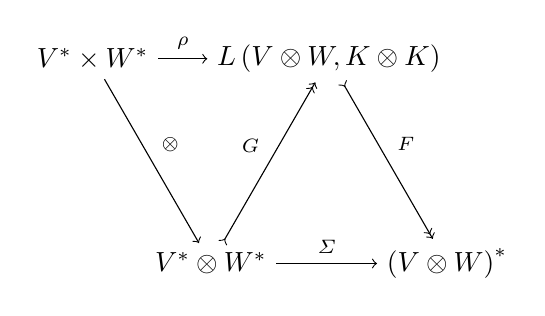
\begin{tikzpicture}[auto] 
    \node (a) at (0, 2.60) {$V^* \times W^* $};
    \node (b) at (1.5, 0) {$V^* \otimes W^* $};
    \node (c) at (3, 2.60) {$L\left( V\otimes W,K\otimes K \right) $};
    \node (d) at (4.5, 0) {$\left( V\otimes W\right)^* $};
    \draw [->] (a) to node {$\scriptstyle \otimes $} (b);
    \draw [->] (a) to node {$\scriptstyle \rho $} (c);
    \draw [>->>] (b) to node {$\scriptstyle G$} (c);
    \draw [->] (b) to node {$\scriptstyle \varSigma $} (d);
    \draw [>->>] (c) to node {$\scriptstyle F$} (d);
  \end{tikzpicture} 
\end{center}
即ち、$\varSigma = F \circ G$とおかれると、その写像$\varSigma$は線形同型写像であり、$\forall(\varphi,\chi) \in V^{*} \times W^{*}\forall\left( \mathbf{v},\mathbf{w} \right) \in V \times W$に対し、次のようになる。
\begin{align*}
\varSigma(\varphi \otimes \chi)\left( \mathbf{v} \otimes \mathbf{w} \right) &= (F \circ G)(\varphi \otimes \chi)\left( \mathbf{v} \otimes \mathbf{w} \right)\\
&= (F \circ G \circ \otimes )(\varphi,\chi)\left( \mathbf{v} \otimes \mathbf{w} \right)\\
&= (F \circ \rho)(\varphi,\chi)\left( \mathbf{v} \otimes \mathbf{w} \right)\\
&= F\left( \rho(\varphi,\chi) \right)\left( \mathbf{v} \otimes \mathbf{w} \right)\\
&= \left( \sigma \circ \rho(\varphi,\chi) \right)\left( \mathbf{v} \otimes \mathbf{w} \right)\\
&= \sigma\left( \rho(\varphi,\chi)\left( \mathbf{v} \otimes \mathbf{w} \right) \right)\\
&= \sigma\left( \varphi\left( \mathbf{v} \right) \otimes \chi\left( \mathbf{w} \right) \right)\\
&= \varphi\left( \mathbf{v} \right)\chi\left( \mathbf{w} \right)
\end{align*}
\end{proof}
\begin{thm}\label{2.4.5.15}
体$K$上の$n$次元vector空間$V$が与えられたとき、組$(V, \cdot )$はそれらのvector空間たち$K$、$V$のtensor積である。なお、$\cdot$はscalar倍である。さらに、ある線形同型写像$\rho:K \otimes V \rightarrow V$が一意的に存在して、$\cdot = \rho \circ \otimes$が成り立ち、その線形同型写像$\rho$は、$\forall\mathbf{v} \in V$に対し、$\rho\left( \alpha \otimes \mathbf{v} \right) = \alpha\mathbf{v}$を満たす。ゆえに、$K \otimes V \cong V$が成り立つ。
\end{thm}
\begin{proof}
体$K$上の$n$次元vector空間$V$が与えられたとき、$\forall k,l \in K\forall\alpha,\beta \in K\forall\mathbf{v} \in V$に対し、次のようになるかつ、
\begin{align*}
(k\alpha + l\beta)\mathbf{v} = k\alpha\mathbf{v} + l\beta\mathbf{v}
\end{align*}
$\forall k,l \in K\forall\alpha \in K\forall\mathbf{v},\mathbf{w} \in V$に対し、次のようになるので、
\begin{align*}
\alpha(kv + lw) = k\alpha\mathbf{v} + l\alpha\mathbf{w}
\end{align*}
scalar倍$\cdot :K \times V \rightarrow V$は双線形写像である。さらに、そのvector空間$V$の基底として$\left\langle \mathbf{v}_{i} \right\rangle_{i \in \varLambda_{n}}$、そのvector空間$K$の基底として$\alpha \neq 0$なるvector$\alpha$が考えられれば、$\sum_{i \in \varLambda_{n}} {c_{i}\alpha\mathbf{v}_{i}} = \mathbf{0}$が成り立つなら、両辺に$\alpha$で割ることで$\sum_{i \in \varLambda_{n}} {c_{i}\mathbf{v}_{i}} = \mathbf{0}$が得られる。仮定より$\forall i \in \varLambda_{n}$に対し、$c_{i} = 0$が得られるかつ、$\forall\mathbf{v} \in V$に対し、$\mathbf{v} = \sum_{i \in \varLambda_{n}} {v_{i}\mathbf{v}_{i}}$とおかれれば、$\alpha \neq 0$に注意して$\mathbf{v} = \sum_{i \in \varLambda_{n}} {\frac{v_{i}}{\alpha}\alpha\mathbf{v}_{i}}$が得られるので、その組$\left\langle \alpha\mathbf{v}_{i} \right\rangle_{i \in \varLambda_{n}}$もそのvector空間$V$の基底となる。定理\ref{2.4.5.2}よりその組$(V, \cdot )$はそれらのvector空間たち$K$、$V$のtensor積である。\par
さらに、$\forall\mathbf{v} \in V$に対し、$\rho\left( \alpha \otimes \mathbf{v} \right) = \alpha\mathbf{v}$を満たすような線形写像$\rho:K \otimes V \rightarrow V$が考えられれば、$\forall\left( k,\mathbf{v} \right) \in K \times V$に対し、$\mathbf{v} = \sum_{i \in \varLambda_{n}} {k_{i}\mathbf{v}_{i}}$とおかれれば、次のようになることから、
\begin{align*}
\cdot \left( k,\mathbf{v} \right) &= k\mathbf{v} = \frac{k}{\alpha}\alpha\sum_{i \in \varLambda_{n}} {k_{i}\mathbf{v}_{i}}\\
&= \sum_{i \in \varLambda_{n}} {\frac{kk_{i}}{\alpha}\alpha\mathbf{v}_{i}}\\
&= \sum_{i \in \varLambda_{n}} {\frac{kk_{i}}{\alpha}\rho\left( \alpha \otimes \mathbf{v}_{i} \right)}\\
&= \sum_{i \in \varLambda_{n}} {\rho\left( k \otimes k_{i}\mathbf{v}_{i} \right)}\\
&= \rho\left( k \otimes \sum_{i \in \varLambda_{n}} {k_{i}\mathbf{v}_{i}} \right)\\
&= \rho\left( k \otimes \mathbf{v} \right)\\
&= \rho \circ \otimes \left( k,\mathbf{v} \right)
\end{align*}
ある線形写像$\rho:K \otimes V \rightarrow V$が存在して、$\cdot = \rho \circ \otimes$が成り立つ。そこで、定理\ref{2.4.5.3}よりその線形写像$\rho$は線形同型写像でありその存在は一意的である。ゆえに、$K \otimes V \cong V$が成り立つ。
\end{proof}
\begin{thm}\label{2.4.5.16}
体$K$が与えられたとき、組$(K, \cdot )$はそれらのvector空間たち$K$同士のtensor積である。さらに、ある線形同型写像$\rho:K \otimes K\overset{\sim}{\rightarrow}K$が一意的に存在して、$\cdot = \rho \circ \otimes$が成り立ち、その線形同型写像$\rho$は$\rho(\alpha \otimes \beta) = \alpha\beta$を満たす。ゆえに、$K \otimes K \cong K$が成り立つ。
\end{thm}
\begin{proof} 定理\ref{2.4.5.15}より明らかである。
\end{proof}
\begin{thm}\label{2.4.5.17}
体$K$上の$m$次元vector空間$V$、$n$次元vector空間$W$が与えられたとき、ある線形同型写像$\rho:V \otimes W\overset{\sim}{\rightarrow}W \otimes V$が一意的に存在して、その線形同型写像$\rho$は、$\forall\left( \mathbf{v},\mathbf{w} \right) \in V \times W$に対し、$\rho\left( \mathbf{v} \otimes \mathbf{w} \right) = \mathbf{w} \otimes \mathbf{v}$を満たす。ゆえに、$V \otimes W \cong W \otimes V$が成り立つ。
\end{thm}
\begin{proof}
体$K$上の$m$次元vector空間$V$、$n$次元vector空間$W$、これらの基底たちそれぞれ$\left\langle \mathbf{v}_{i} \right\rangle_{i \in \varLambda_{m}}$、$\left\langle \mathbf{w}_{j} \right\rangle_{j \in \varLambda_{n}}$が与えられたとき、定理\ref{2.4.5.2}よりそれらのvector空間たち$V \otimes W$、$W \otimes V$の基底たちがそれぞれ$\left\langle \mathbf{v}_{i} \otimes \mathbf{w}_{j} \right\rangle_{(i,j) \in \varLambda_{m} \times \varLambda_{n}}$、$\left\langle \mathbf{w}_{j} \otimes \mathbf{v}_{i} \right\rangle_{(i,j) \in \varLambda_{m} \times \varLambda_{n}}$と与えられる。したがって、$\forall\left( \mathbf{v},\mathbf{w} \right) \in V \times W$に対し、$\rho\left( \mathbf{v} \otimes \mathbf{w} \right) = \mathbf{w} \otimes \mathbf{v}$を満たすような線形写像$\rho:V \otimes W \rightarrow W \otimes V$が考えられれば、$\forall\mathbf{v} \in V\forall\mathbf{w} \in W$に対し、$\mathbf{v} = \sum_{i \in \varLambda_{m}} {k_{i}\mathbf{v}_{i}}$、$\mathbf{w} = \sum_{j \in \varLambda_{n}} {l_{j}\mathbf{w}_{j}}$として、次のようになることから、
\begin{align*}
\mathbf{w} \otimes \mathbf{v} &= \sum_{j \in \varLambda_{n}} {l_{j}\mathbf{w}_{j}} \otimes \sum_{i \in \varLambda_{m}} {k_{i}\mathbf{v}_{i}}\\
&= \sum_{i \in \varLambda_{m}} {\sum_{j \in \varLambda_{n}} {k_{i}l_{j}\mathbf{w}_{j} \otimes \mathbf{v}_{i}}}\\
&= \sum_{i \in \varLambda_{m}} {\sum_{j \in \varLambda_{n}} {k_{i}l_{j}\rho\left( \mathbf{v}_{i} \otimes \mathbf{w}_{j} \right)}}\\
&= \rho\left( \sum_{i \in \varLambda_{m}} {k_{i}\mathbf{v}_{i}} \otimes \sum_{j \in \varLambda_{n}} {l_{j}\mathbf{w}_{j}} \right)\\
&= \rho\left( \mathbf{v} \otimes \mathbf{w} \right)
\end{align*}
定理\ref{2.4.5.3}よりその線形写像$\rho$は線形同型写像でありその存在は一意的である。ゆえに、$V \otimes W \cong W \otimes V$が成り立つ。
\end{proof}
\begin{thm}\label{2.4.5.18}
体$K$上の$m$次元vector空間$U$、$n$次元vector空間$V$、$o$次元vector空間$W$が与えられたとき、次式が成り立つ。
\begin{align*}
L(U,W;W) \cong L(U \otimes V,W)
\end{align*}
このとき、ある線形同型写像$\otimes^{*}:L(U \otimes V,W)\overset{\sim}{\rightarrow}L(U,W;W)$が存在して、$\otimes^{*}(\rho) = \rho \circ \otimes$が成り立ち、$\otimes^{*}(\rho):U \times V \rightarrow W;\left( \mathbf{u},\mathbf{v} \right) \mapsto \rho\left( \mathbf{u} \otimes \mathbf{v} \right)$が成り立つ。
\end{thm}
\begin{proof}
体$K$上の$m$次元vector空間$U$、$n$次元vector空間$V$、$o$次元vector空間$W$が与えられたとき、$\otimes^{*}(\rho) = \rho \circ \otimes$なる写像$\otimes^{*}:L(U \otimes V,W) \rightarrow L(U,W;W)$が考えられれば、$\forall k,l \in K\forall\rho,\sigma \in L(U \otimes V,W)\forall\left( \mathbf{u},\mathbf{v} \right) \in U \times V$に対し、次のようになる。
\begin{align*}
\otimes^{*}(k\rho + l\sigma)\left( \mathbf{u},\mathbf{v} \right) &= (k\rho + l\sigma) \circ \otimes \left( \mathbf{u},\mathbf{v} \right)\\
&= (k\rho + l\sigma)\left( \mathbf{u} \otimes \mathbf{v} \right)\\
&= k\rho\left( \mathbf{u} \otimes \mathbf{v} \right) + l\sigma\left( \mathbf{u} \otimes \mathbf{v} \right)\\
&= k\rho \circ \otimes \left( \mathbf{u},\mathbf{v} \right) + l\sigma \circ \otimes \left( \mathbf{u},\mathbf{v} \right)\\
&= k \otimes^{*}(\rho)\left( \mathbf{u},\mathbf{v} \right) + l \otimes^{*}(\rho)\left( \mathbf{u},\mathbf{v} \right)\\
&= \left( k \otimes^{*}(\rho) + l \otimes^{*}(\rho) \right)\left( \mathbf{u},\mathbf{v} \right)
\end{align*}
これにより、その写像$\otimes^{*}$は線形写像である。\par
一方で、$\forall\varPhi \in L(U,V;W)$に対し、定理\ref{2.4.5.3}よりある線形写像$\rho:U \otimes V \rightarrow W$が一意的に存在して、$\varPhi = \rho \circ \otimes$が成り立つので、写像$\otimes':L(U,W;W) \rightarrow L(U \otimes V,W);\varPhi \mapsto \rho$が定義されることができる。このとき、$\forall\varPhi \in L(U,V;W)$に対し、次のようになるかつ、
\begin{align*}
\otimes^{*} \circ \otimes'(\varPhi) = \otimes^{*}\left( \otimes'(\varPhi) \right) = \otimes^{*}(\rho) = \rho \circ \otimes = \varPhi
\end{align*}
$\forall\rho \in L(U \otimes V,W)$に対し、次のようになるので、
\begin{align*}
\otimes' \circ \otimes^{*}(\rho) = \otimes'\left( \otimes^{*}(\rho) \right) = \otimes'(\rho \circ \otimes ) = \rho
\end{align*}
$\otimes^{*} \circ \otimes' = I_{L(U,V;W)}$かつ$\otimes' \circ \otimes^{*} = I_{L(U \otimes V,W)}$が成り立つことになり、したがって、$\otimes' = {\otimes^{*}}^{- 1}$が得られる。これにより、その線形写像$\otimes^{*}$は線形同型写像である。
\end{proof}
\begin{thm}\label{2.4.5.19}
体$K$上の$m$次元vector空間$U$、$n$次元vector空間$V$、$o$次元vector空間$W$が与えられたとき、次式が成り立つ。
\begin{align*}
L(U,V;W) \cong \left( U^{*} \otimes V^{*} \right) \otimes W
\end{align*}
このとき、ある線形同型写像$\varSigma:\left( U^{*} \otimes V^{*} \right) \otimes W\overset{\sim}{\rightarrow}L(U,V;W)$が存在して、$\forall(f,g) \in U^{*} \times V^{*}\forall\left( \mathbf{u},\mathbf{v} \right) \in U \times V\forall\mathbf{w} \in W$に対し、$\varSigma\left( (f \otimes g) \otimes \mathbf{w} \right)\left( \mathbf{u},\mathbf{v} \right) = f\left( \mathbf{u} \right)g\left( \mathbf{v} \right)\mathbf{w}$が成り立つ。
\end{thm}
\begin{proof}
体$K$上の$m$次元vector空間$U$、$n$次元vector空間$V$、$o$次元vector空間$W$が与えられたとき、定理\ref{2.4.5.18}よりある線形同型写像$\otimes^{*}:L(U \otimes V,W)\overset{\sim}{\rightarrow}L(U,V;W)$が存在して、$\otimes^{*}(\rho) = \rho \circ \otimes$が成り立つ。また、定理\ref{2.4.5.7}よりそのvector空間$L(U \otimes V,W)$とそのvector空間$W$のvectorのその双対空間$(U \otimes V)^{*}$の線形形式の像倍へ写す双線形写像$\psi_{U \otimes V,W}$との組$\left( L(U \otimes V,W),\psi_{U \otimes V,W} \right)$はそれらのvector空間たち$W$、$(U \otimes V)^{*}$のtensor積であり、ある線形同型写像$\rho:W \otimes (U \otimes V)^{*}\overset{\sim}{\rightarrow}L(U \otimes V,W)$が存在して、$\psi_{U \otimes V,W} = \rho \circ \otimes$が成り立つ。そこで、定理\ref{2.4.5.17}よりある線形同型写像$\sigma:(U \otimes V)^{*} \otimes W\overset{\sim}{\rightarrow}W \otimes (U \otimes V)^{*}$が一意的に存在して、その線形同型写像$\sigma$は、$\forall\left( \tau,\mathbf{w} \right) \in (U \otimes V)^{*} \times W$に対し、$\sigma\left( \tau \otimes \mathbf{w} \right) = \mathbf{w} \otimes \tau$を満たす。以上の議論により、次のようになる。
\begin{center}
  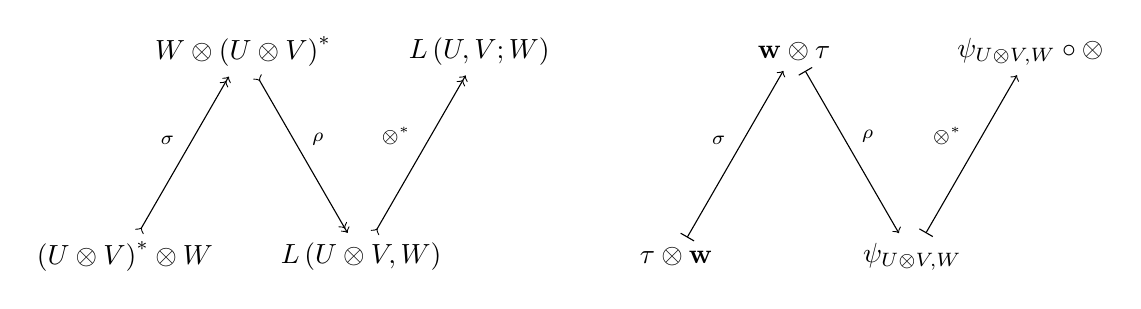
\begin{tikzpicture}[auto] 
    %\node (f) at (8.50, 2.60) {$ $};
    \node (g) at (8.50,    0) {$\tau \otimes {\bf w} $};
    \node (h) at (10.0, 2.60) {${\bf w} \otimes \tau $};
    \node (i) at (11.5,    0) {$\psi_{U\otimes V,W} $};
    \node (j) at (13.0, 2.60) {$\psi_{U\otimes V,W} \circ \otimes $};
    %\draw [|->] (f) to node {$\scriptstyle $} (g);
    \draw [|->] (g) to node {$\scriptstyle \sigma $} (h);
    \draw [|->] (h) to node {$\scriptstyle \rho $} (i);
    \draw [|->] (i) to node {$\scriptstyle \otimes^* $} (j);
    %\node (a) at (0.00, 2.60) {$ $};
    \node (b) at (1.50,    0) {$\left( U\otimes V\right)^* \otimes W$};
    \node (c) at (3.00, 2.60) {$W\otimes \left( U\otimes V\right)^* $};
    \node (d) at (4.50,    0) {$L\left( U\otimes V,W\right) $};
    \node (e) at (6.00, 2.60) {$L\left( U,V;W\right) $};
    %\draw [>->>] (a) to node {$\scriptstyle $} (b);
    \draw [>->>] (b) to node {$\scriptstyle \sigma $} (c);
    \draw [>->>] (c) to node {$\scriptstyle \rho $} (d);
    \draw [>->>] (d) to node {$\scriptstyle \otimes^* $} (e);
  \end{tikzpicture} 
\end{center}
また、定理\ref{2.4.5.14}よりある線形同型写像$\varSigma':V^{*} \otimes W^{*}\overset{\sim}{\rightarrow}(V \otimes W)^{*}$が存在して、$\forall(\varphi,\chi) \in U^{*} \times V^{*}\forall\left( \mathbf{u},\mathbf{v} \right) \in U \times V$に対し、$\varSigma'(\varphi \otimes \chi)\left( \mathbf{u} \otimes \mathbf{v} \right) = \varphi\left( \mathbf{u} \right)\chi\left( \mathbf{v} \right)$が成り立つ。\par
そこで、$\forall(f,g) \in U^{*} \times V^{*}\forall\mathbf{w} \in W$に対し、$T\left( (f \otimes g) \otimes \mathbf{w} \right) = \varSigma'(f \otimes g) \otimes \mathbf{w}$が成り立つような写像$T:\left( U^{*} \otimes V^{*} \right) \otimes W \rightarrow (U \otimes V)^{*} \otimes W$が考えられよう。$\forall\left( \tau,\mathbf{w} \right) \in (U \otimes V)^{*} \times W$に対し、$\varUpsilon\left( \tau \otimes \mathbf{w} \right) = {\varSigma'}^{- 1}(\tau) \otimes \mathbf{w}$が成り立つような写像$\varUpsilon:(U \otimes V)^{*} \otimes W \rightarrow \left( U^{*} \otimes V^{*} \right) \otimes W$が考えられれば、$\forall\mathbf{T} \in \left( U^{*} \otimes V^{*} \right) \otimes W$に対し、それらのvector空間たち$U^{*}$、$V^{*}$、$W$の基底たちそれぞれ$\left\langle \lambda_{h} \right\rangle_{h \in \varLambda_{m}}$、$\left\langle \mu_{i} \right\rangle_{i \in \varLambda_{n}}$、$\left\langle \mathbf{w}_{j} \right\rangle_{j \in \varLambda_{o}}$を用いれば、定理\ref{2.4.5.2}よりその組$\left\langle \lambda_{h} \otimes \mu_{i} \right\rangle_{(h,i) \in \varLambda_{m} \times \varLambda_{n}}$がそのvector空間$U^{*} \otimes V^{*}$の基底をなすので、次のようにおかれることができて、
\begin{align*}
\mathbf{T} = \sum_{(h,i,j) \in \varLambda_{m} \times \varLambda_{n} \times \varLambda_{o}} {\xi_{hij}\left( \lambda_{h} \otimes \mu_{i} \right) \otimes \mathbf{w}_{j}}
\end{align*}
このとき、次のようになる。
\begin{align*}
\varUpsilon \circ T\left( \mathbf{T} \right) &= \varUpsilon \circ T\left( \sum_{(h,i,j) \in \varLambda_{m} \times \varLambda_{n} \times \varLambda_{o}} {\xi_{hij}\left( \lambda_{h} \otimes \mu_{i} \right) \otimes \mathbf{w}_{j}} \right)\\
&= \sum_{(h,i,j) \in \varLambda_{m} \times \varLambda_{n} \times \varLambda_{o}} {\xi_{hij}\varUpsilon \circ T\left( \left( \lambda_{h} \otimes \mu_{i} \right) \otimes \mathbf{w}_{j} \right)}\\
&= \sum_{(h,i,j) \in \varLambda_{m} \times \varLambda_{n} \times \varLambda_{o}} {\xi_{hij}\varUpsilon\left( T\left( \left( \lambda_{h} \otimes \mu_{i} \right) \otimes \mathbf{w}_{j} \right) \right)}\\
&= \sum_{(h,i,j) \in \varLambda_{m} \times \varLambda_{n} \times \varLambda_{o}} {\xi_{hij}\varUpsilon\left( \varSigma'\left( \lambda_{h} \otimes \mu_{i} \right) \otimes \mathbf{w}_{j} \right)}\\
&= \sum_{(h,i,j) \in \varLambda_{m} \times \varLambda_{n} \times \varLambda_{o}} {\xi_{hij}{\varSigma'}^{- 1} \circ \varSigma'\left( \lambda_{h} \otimes \mu_{i} \right) \otimes \mathbf{w}_{j}}\\
&= \sum_{(h,i,j) \in \varLambda_{m} \times \varLambda_{n} \times \varLambda_{o}} {\xi_{hij}\left( \lambda_{h} \otimes \mu_{i} \right) \otimes \mathbf{w}_{j}} = \mathbf{T}
\end{align*}
一方で、$\forall\mathbf{U} \in (U \otimes V)^{*} \otimes W$に対し、定理\ref{2.4.5.2}より次のようにおかれることができて、
\begin{align*}
\mathbf{U} = \sum_{(h,i,j) \in \varLambda_{m} \times \varLambda_{n} \times \varLambda_{o}} {o_{hij}\tau_{hi} \otimes \mathbf{w}_{j}}
\end{align*}
このとき、次のようになる。
\begin{align*}
T \circ \varUpsilon\left( \mathbf{U} \right) &= T \circ \varUpsilon\left( \sum_{(h,i,j) \in \varLambda_{m} \times \varLambda_{n} \times \varLambda_{o}} {o_{hij}\tau_{hi} \otimes \mathbf{w}_{j}} \right)\\
&= \sum_{(h,i,j) \in \varLambda_{m} \times \varLambda_{n} \times \varLambda_{o}} {o_{hij}T \circ \varUpsilon\left( \tau_{hi} \otimes \mathbf{w}_{j} \right)}\\
&= \sum_{(h,i,j) \in \varLambda_{m} \times \varLambda_{n} \times \varLambda_{o}} {o_{hij}T\left( \varUpsilon\left( \tau_{hi} \otimes \mathbf{w}_{j} \right) \right)}\\
&= \sum_{(h,i,j) \in \varLambda_{m} \times \varLambda_{n} \times \varLambda_{o}} {o_{hij}T\left( {\varSigma'}^{- 1}\left( \tau_{hi} \right) \otimes \mathbf{w}_{j} \right)}\\
&= \sum_{(h,i,j) \in \varLambda_{m} \times \varLambda_{n} \times \varLambda_{o}} {o_{hij}\varSigma' \circ {\varSigma'}^{- 1}\left( \tau_{hi} \right) \otimes \mathbf{w}_{j}}\\
&= \sum_{(h,i,j) \in \varLambda_{m} \times \varLambda_{n} \times \varLambda_{o}} {o_{hij}\tau_{hi} \otimes \mathbf{w}_{j}} = \mathbf{U}
\end{align*}
以上より、$\varUpsilon = T^{- 1}$が得られたので、その線形写像$T$は線形同型写像である。\par
以上の議論により次のようになる。
\begin{center}
  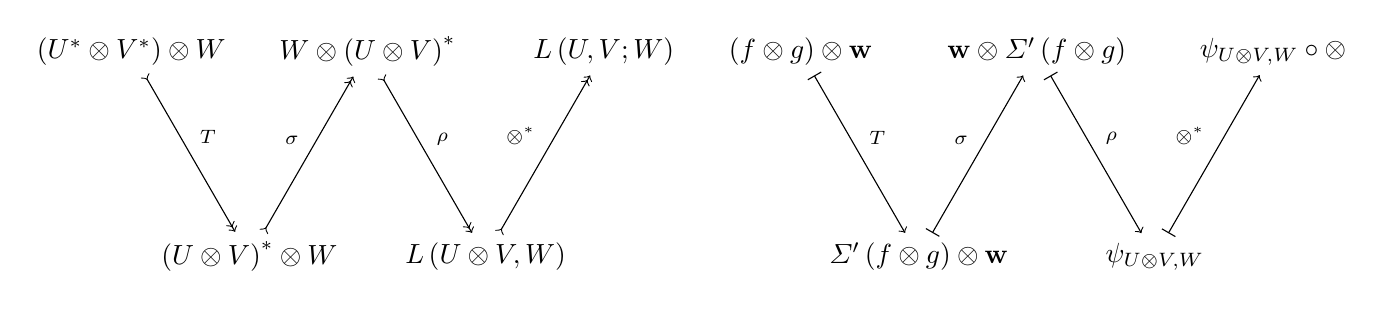
\begin{tikzpicture}[auto] 
    \node (f) at (8.50, 2.60) {$\left( f\otimes g\right) \otimes {\bf w} $};
    \node (g) at (10.0,    0) {$\varSigma' \left( f\otimes g\right) \otimes {\bf w} $};
    \node (h) at (11.5, 2.60) {${\bf w} \otimes \varSigma' \left( f\otimes g\right) $};
    \node (i) at (13.0,    0) {$\psi_{U\otimes V,W} $};
    \node (j) at (14.5, 2.60) {$\psi_{U\otimes V,W} \circ \otimes $};
    \draw [|->] (f) to node {$\scriptstyle T$} (g);
    \draw [|->] (g) to node {$\scriptstyle \sigma $} (h);
    \draw [|->] (h) to node {$\scriptstyle \rho $} (i);
    \draw [|->] (i) to node {$\scriptstyle \otimes^* $} (j);
    \node (a) at (0.00, 2.60) {$\left( U^* \otimes V^* \right) \otimes W$};
    \node (b) at (1.50,    0) {$\left( U\otimes V\right)^* \otimes W$};
    \node (c) at (3.00, 2.60) {$W\otimes \left( U\otimes V\right)^* $};
    \node (d) at (4.50,    0) {$L\left( U\otimes V,W\right) $};
    \node (e) at (6.00, 2.60) {$L\left( U,V;W\right) $};
    \draw [>->>] (a) to node {$\scriptstyle T $} (b);
    \draw [>->>] (b) to node {$\scriptstyle \sigma $} (c);
    \draw [>->>] (c) to node {$\scriptstyle \rho $} (d);
    \draw [>->>] (d) to node {$\scriptstyle \otimes^* $} (e);
  \end{tikzpicture} 
\end{center}
そこで、次式のように線形同型写像$\varSigma:\left( U^{*} \times V^{*} \right) \otimes W \rightarrow L(U,V;W)$がおかれ、
\begin{center}
  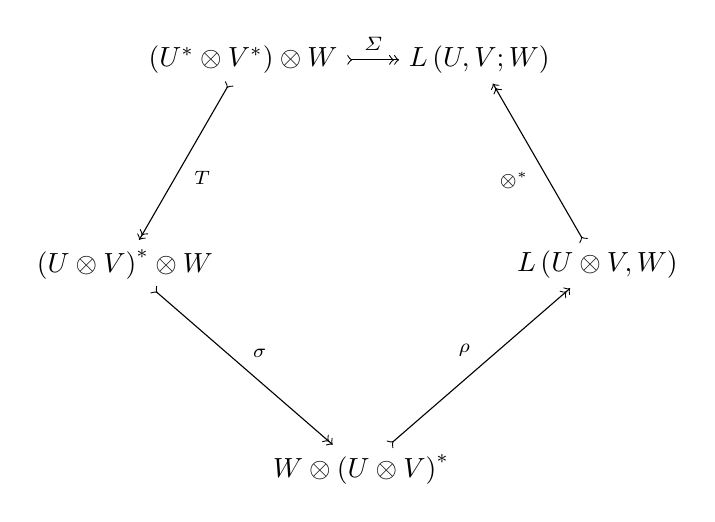
\begin{tikzpicture}[auto] 
    \node (a) at (1.50, 5.20) {$\left( U^* \otimes V^* \right) \otimes W$};
    \node (b) at (0.00, 2.60) {$\left( U\otimes V\right)^* \otimes W$};
    \node (c) at (3.00,    0) {$W\otimes \left( U\otimes V\right)^* $};
    \node (d) at (6.00, 2.60) {$L\left( U\otimes V,W\right) $};
    \node (e) at (4.50, 5.20) {$L\left( U,V;W\right) $};
    \draw [>->>] (a) to node {$\scriptstyle T $} (b);
    \draw [>->>] (b) to node {$\scriptstyle \sigma $} (c);
    \draw [>->>] (c) to node {$\scriptstyle \rho $} (d);
    \draw [>->>] (d) to node {$\scriptstyle \otimes^* $} (e);
    \draw [>->>] (a) to node {$\scriptstyle \varSigma $} (e);
  \end{tikzpicture} 
\end{center}
$\forall(f,g) \in U^{*} \times V^{*}\forall\left( \mathbf{u},\mathbf{v} \right) \in U \times V\forall\mathbf{w} \in W$に対し、次のようにおくと、
\begin{align*}
f = \sum_{h \in \varLambda_{m}} {k_{h}\lambda_{h}},\ \ g = \sum_{i \in \varLambda_{n}} {l_{i}\mu_{i}},\ \ \mathbf{w} = \sum_{j \in \varLambda_{o}} {m_{j}\mathbf{w}_{j}}
\end{align*}
$\forall h \in \varLambda_{m}\forall i \in \varLambda_{n}\forall j \in \varLambda_{o}\forall\left( \mathbf{u},\mathbf{v} \right) \in U \times V$に対し、次のようになるので、
\begin{align*}
\varSigma\left( \left( \lambda_{h} \otimes \mu_{i} \right) \otimes \mathbf{w}_{j} \right)\left( \mathbf{u},\mathbf{v} \right) &= \left( \otimes^{*} \circ \rho \circ \sigma \circ T \right)\left( \left( \lambda_{h} \otimes \mu_{i} \right) \otimes \mathbf{w}_{j} \right)\left( \mathbf{u},\mathbf{v} \right)\\
&= \otimes^{*}\left( \rho\left( \sigma\left( T\left( \left( \lambda_{h} \otimes \mu_{i} \right) \otimes \mathbf{w}_{j} \right) \right) \right) \right)\left( \mathbf{u},\mathbf{v} \right)\\
&= \otimes^{*}\left( \rho\left( \sigma\left( \varSigma'\left( \lambda_{h} \otimes \mu_{i} \right) \otimes \mathbf{w}_{j} \right) \right) \right)\left( \mathbf{u},\mathbf{v} \right)\\
&= \otimes^{*}\left( \rho\left( \mathbf{w}_{j} \otimes \varSigma'\left( \lambda_{h} \otimes \mu_{i} \right) \right) \right)\left( \mathbf{u},\mathbf{v} \right)\\
&= \otimes^{*}\left( \rho \circ \otimes \left( \mathbf{w}_{j},\varSigma'\left( \lambda_{h} \otimes \mu_{i} \right) \right) \right)\left( \mathbf{u},\mathbf{v} \right)\\
&= \otimes^{*}\left( \psi_{U \otimes V,W}\left( \mathbf{w}_{j},\varSigma'\left( \lambda_{h} \otimes \mu_{i} \right) \right) \right)\left( \mathbf{u},\mathbf{v} \right)\\
&= \left( \psi_{U \otimes V,W}\left( \mathbf{w}_{j},\varSigma'\left( \lambda_{h} \otimes \mu_{i} \right) \right) \right) \circ \otimes \left( \mathbf{u},\mathbf{v} \right)\\
&= \left( \psi_{U \otimes V,W}\left( \mathbf{w}_{j},\varSigma'\left( \lambda_{h} \otimes \mu_{i} \right) \right) \right)\left( \mathbf{u} \otimes \mathbf{v} \right)\\
&= \varSigma'\left( \lambda_{h} \otimes \mu_{i} \right)\left( \mathbf{u} \otimes \mathbf{v} \right)\mathbf{w}_{j}\\
&= \lambda_{h}\left( \mathbf{u} \right)\mu_{i}\left( \mathbf{v} \right)\mathbf{w}_{j}
\end{align*}
$\forall\left( \mathbf{u},\mathbf{v} \right) \in U \times V$に対し、次のようになる。
\begin{align*}
\varSigma\left( (f \otimes g) \otimes \mathbf{w} \right)\left( \mathbf{u},\mathbf{v} \right) &= \varSigma\left( \left( \sum_{h \in \varLambda_{m}} {k_{h}\lambda_{h}} \otimes \sum_{i \in \varLambda_{n}} {l_{i}\mu_{i}} \right) \otimes \sum_{j \in \varLambda_{o}} {m_{j}\mathbf{w}_{j}} \right)\left( \mathbf{u},\mathbf{v} \right)\\
&= \sum_{h \in \varLambda_{m}} {\sum_{i \in \varLambda_{n}} {\sum_{j \in \varLambda_{o}} {k_{h}l_{i}m_{j}\varSigma\left( \left( \lambda_{h} \otimes \mu_{i} \right) \otimes \mathbf{w}_{j} \right)\left( \mathbf{u},\mathbf{v} \right)}}}\\
&= \sum_{h \in \varLambda_{m}} {\sum_{i \in \varLambda_{n}} {\sum_{j \in \varLambda_{o}} {k_{h}l_{i}m_{j}\lambda_{h}\left( \mathbf{u} \right)\mu_{i}\left( \mathbf{v} \right)\mathbf{w}_{j}}}}\\
&= \sum_{h \in \varLambda_{m}} {k_{h}\lambda_{h}\left( \mathbf{u} \right)}\sum_{i \in \varLambda_{n}} {l_{i}\mu_{i}\left( \mathbf{v} \right)}\sum_{j \in \varLambda_{o}} {m_{j}\mathbf{w}_{j}}\\
&= f\left( \mathbf{u} \right)g\left( \mathbf{v} \right)\mathbf{w}
\end{align*}
よって、ある線形同型写像$\varSigma:\left( U^{*} \otimes V^{*} \right) \otimes W\overset{\sim}{\rightarrow}L(U,V;W)$が存在して、$\forall(f,g) \in U^{*} \times V^{*}\forall\left( \mathbf{u},\mathbf{v} \right) \in U \times V\forall\mathbf{w} \in W$に対し、$\varSigma\left( (f \otimes g) \otimes \mathbf{w} \right)\left( \mathbf{u},\mathbf{v} \right) = f\left( \mathbf{u} \right)g\left( \mathbf{v} \right)\mathbf{w}$が成り立つ。
\end{proof}
\begin{thm}\label{2.4.5.20}
体$K$上の$m$次元vector空間$U$、$n$次元vector空間$V$、$o$次元vector空間$W$が与えられたとき、次式が成り立つ。
\begin{align*}
L\left( U,L(V,W) \right) \cong \left( U^{*} \otimes V^{*} \right) \otimes W
\end{align*}
このとき、ある線形同型写像$\varSigma:\left( U^{*} \otimes V^{*} \right) \otimes W\overset{\sim}{\rightarrow}L\left( U,L(V,W) \right)$が存在して、$\forall(f,g) \in U^{*} \times V^{*}\forall\mathbf{u} \in U\forall\mathbf{w} \in W$に対し、$\varSigma\left( (f \otimes g) \otimes \mathbf{w} \right)\left( \mathbf{u} \right) = \left( V \rightarrow W;\mathbf{v} \mapsto f\left( \mathbf{u} \right)g\left( \mathbf{v} \right)\mathbf{w} \right)$が成り立つ。
\end{thm}
\begin{proof}
体$K$上の$m$次元vector空間$U$、$n$次元vector空間$V$、$o$次元vector空間$W$が与えられたとき、$\forall\left( f,g,\mathbf{w} \right) \in U^{*} \times V^{*} \times W$に対し、$T\left( (f \otimes g) \otimes \mathbf{w} \right) = \left( \mathbf{w} \otimes g \right) \otimes f$を満たすような線形写像$\rho:\left( U^{*} \otimes V^{*} \right) \otimes W \rightarrow \left( W \otimes V^{*} \right) \otimes U^{*}$が考えられれば、$\forall\mathbf{T} \in \left( W \otimes V^{*} \right) \otimes U^{*}$に対し、それらのvector空間たち$U^{*}$、$V^{*}$、$W$の基底たちそれぞれ$\left\langle \lambda_{h} \right\rangle_{h \in \varLambda_{m}}$、$\left\langle \mu_{i} \right\rangle_{i \in \varLambda_{n}}$、$\left\langle \mathbf{w}_{j} \right\rangle_{j \in \varLambda_{o}}$を用いれば、定理\ref{2.4.5.2}よりその組$\left\langle \left( \mathbf{w}_{j} \otimes \mu_{i} \right) \otimes \lambda_{h} \right\rangle_{(h,i,j) \in \varLambda_{m} \times \varLambda_{n} \times \varLambda_{o}}$がそのvector空間$\left( W \otimes V^{*} \right) \otimes U^{*}$の基底をなすので、次のようにおかれることができて、
\begin{align*}
\mathbf{T} = \sum_{(h,i,j) \in \varLambda_{m} \times \varLambda_{n} \times \varLambda_{o}} {\xi_{hij}\left( \mathbf{w}_{j} \otimes \mu_{i} \right) \otimes \lambda_{h}}
\end{align*}
このとき、次のようになる。
\begin{align*}
\mathbf{T} &= \sum_{(h,i,j) \in \varLambda_{m} \times \varLambda_{n} \times \varLambda_{o}} {\xi_{hij}\left( \mathbf{w}_{j} \otimes \mu_{i} \right) \otimes \lambda_{h}}\\
&= \sum_{(h,i,j) \in \varLambda_{m} \times \varLambda_{n} \times \varLambda_{o}} {\xi_{hij}T\left( \left( \lambda_{h} \otimes \mu_{i} \right) \otimes \mathbf{w}_{j} \right)}\\
&= T\left( \sum_{(h,i,j) \in \varLambda_{m} \times \varLambda_{n} \times \varLambda_{o}} {\xi_{hij}\left( \lambda_{h} \otimes \mu_{i} \right) \otimes \mathbf{w}_{j}} \right)
\end{align*}
ゆえに、その線形写像$T$は全射であり、さらに、次のようになるので、
\begin{align*}
\dim{\left( U^{*} \otimes V^{*} \right) \otimes W} &= \dim{U^{*} \otimes V^{*}}\dim W\\
&= \dim U^{*}\dim V^{*}\dim W\\
&= \dim W\dim V^{*}\dim U^{*}\\
&= \dim{W \otimes V^{*}}\dim U^{*}\\
&= \dim{\left( W \otimes V^{*} \right) \otimes U^{*}}
\end{align*}
定理\ref{2.1.5.16}よりその線形写像$T$は線形同型写像である。\par
定理\ref{2.4.5.7}よりある線形同型写像$\rho:W \otimes V^{*} \rightarrow L(V,W)$が存在して、$\forall\left( \mathbf{w},f \right) \in W \times V^{*}$に対し、$\rho\left( \mathbf{w} \otimes f \right):V \rightarrow W;\mathbf{v} \mapsto f\left( \mathbf{v} \right)\mathbf{w}$が成り立つ。そこで、$\forall\left( f,g,\mathbf{w} \right) \in U^{*} \times V^{*} \times W$に対し、$\varSigma'\left( \left( \mathbf{w} \otimes g \right) \otimes f \right) = \rho\left( \mathbf{w} \otimes g \right) \otimes f$を満たすような線形写像$\varSigma':\left( W \otimes V^{*} \right) \otimes U^{*} \rightarrow L(V,W) \otimes U^{*}$が考えられれば、$\forall\mathbf{T} \in L(V,W) \otimes U^{*}$に対し、定理\ref{2.1.2.9}よりそれらのvector空間たち$U^{*}$、$L(V,W)$の基底たちそれぞれ$\left\langle \lambda_{h} \right\rangle_{h \in \varLambda_{m}}$、$\left\langle \varphi_{ij}:V \rightarrow W \right\rangle_{(i,j) \in \varLambda_{n} \times \varLambda_{o}}$を用いれば、定理\ref{2.4.5.2}よりその組$\left\langle \varphi_{ij} \otimes \lambda_{h} \right\rangle_{(h,i,j) \in \varLambda_{m} \times \varLambda_{n} \times \varLambda_{o}}$がそのvector空間$L(V,W) \otimes U^{*}$の基底をなすので、次のようにおくことができる。
\begin{align*}
\mathbf{T} = \sum_{(h,i,j) \in \varLambda_{m} \times \varLambda_{n} \times \varLambda_{o}} {\xi_{hij}\varphi_{ij} \otimes \lambda_{h}}
\end{align*}
このとき、次のようになるので、
\begin{align*}
\mathbf{T} &= \sum_{(h,i,j) \in \varLambda_{m} \times \varLambda_{n} \times \varLambda_{o}} {\xi_{hij}\varphi_{ij} \otimes \lambda_{h}}\\
&= \sum_{(h,i,j) \in \varLambda_{m} \times \varLambda_{n} \times \varLambda_{o}} {\xi_{hij}\rho \circ \rho^{- 1}\left( \varphi_{ij} \right) \otimes \lambda_{h}}\\
&= \sum_{(h,i,j) \in \varLambda_{m} \times \varLambda_{n} \times \varLambda_{o}} {\xi_{hij}\varSigma'\left( \rho^{- 1}\left( \varphi_{ij} \right) \otimes \lambda_{h} \right)}\\
&= \varSigma'\left( \sum_{(h,i,j) \in \varLambda_{m} \times \varLambda_{n} \times \varLambda_{o}} {\xi_{hij}\rho^{- 1}\left( \varphi_{ij} \right) \otimes \lambda_{h}} \right)
\end{align*}
ゆえに、その線形写像$\varSigma'$は全射であり、さらに、次のようになるので、
\begin{align*}
\dim{\left( W \otimes V^{*} \right) \otimes U^{*}} &= \dim{W \otimes V^{*}}\dim U^{*}\\
&= \dim W\dim V^{*}\dim U^{*}\\
&= \dim V\dim W\dim U^{*}\\
&= \dim{L(V,W)}\dim U^{*}\\
&= \dim{L(V,W) \otimes U^{*}}
\end{align*}
定理\ref{2.1.5.16}よりその線形写像$\varSigma'$は線形同型写像である。\par
さらに、定理\ref{2.4.5.7}よりある線形同型写像$\sigma:L(V,W) \otimes U^{*} \rightarrow L\left( U,L(V,W) \right)$が存在して、$\forall(f,g) \in U^{*} \times L(V,W)$に対し、$\sigma(g \otimes f):U \rightarrow L(V,W);\mathbf{u} \mapsto f\left( \mathbf{u} \right)g$が成り立つので、次のようになる。
\begin{center}
  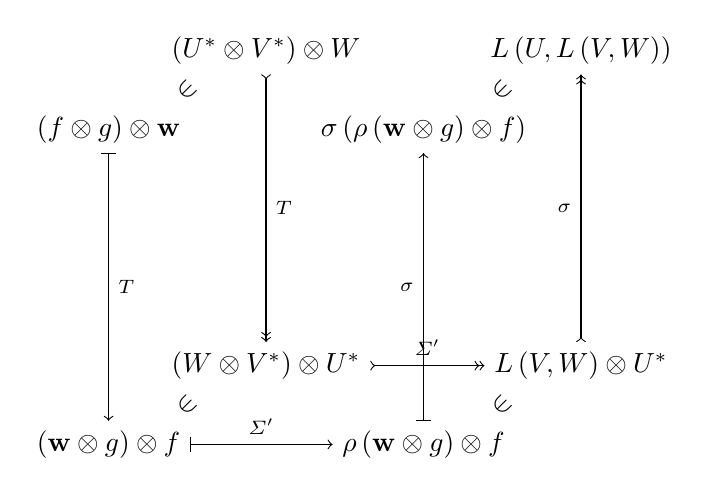
\begin{tikzpicture}[auto] 
    \node (a) at (2.00, 5.00) {$\left( U^* \otimes V^* \right) \otimes W$};
    \node (b) at (2.00, 1.00) {$\left( W\otimes V^* \right) \otimes U^* $};
    \node (c) at (6.00, 1.00) {$L\left( V,W\right) \otimes U^* $};
    \node (d) at (6.00, 5.00) {$L\left( U,L\left( V,W\right) \right) $};
    \draw [>->>] (a) to node {$\scriptstyle T $} (b);
    \draw [>->>] (b) to node {$\scriptstyle \varSigma' $} (c);
    \draw [>->>] (c) to node {$\scriptstyle \sigma $} (d);
    \node (e) at (0.00, 4.00) {$\left( f\otimes g\right) \otimes {\bf w} $};
    \node (f) at (0.00, 0.00) {$\left( {\bf w} \otimes g\right) \otimes f$};
    \node (g) at (4.00, 0.00) {$\rho \left( {\bf w} \otimes g\right) \otimes f$};
    \node (h) at (4.00, 4.00) {$\sigma \left( \rho \left( {\bf w} \otimes g\right) \otimes f\right) $};
    \draw [|->] (e) to node {$\scriptstyle T $} (f);
    \draw [|->] (f) to node {$\scriptstyle \varSigma' $} (g);
    \draw [|->] (g) to node {$\scriptstyle \sigma $} (h);
    \node (i) at (1.00, 0.50) {\rotatebox{45}{$\scriptsize \in $} };
    \node (i) at (5.00, 0.50) {\rotatebox{45}{$\scriptsize \in $} };
    \node (i) at (1.00, 4.50) {\rotatebox{45}{$\scriptsize \in $} };
    \node (i) at (5.00, 4.50) {\rotatebox{45}{$\scriptsize \in $} };
  \end{tikzpicture} 
\end{center}
そこで、次のように線形同型写像$\varSigma:\left( U^{*} \otimes V^{*} \right) \otimes W \rightarrow L\left( U,L(V,W) \right)$がおかれれば、
\begin{center}
  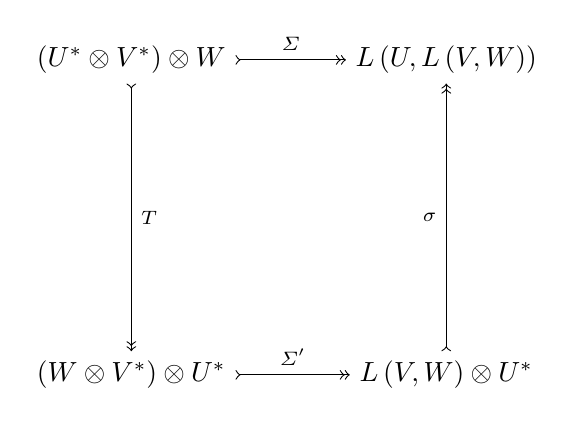
\begin{tikzpicture}[auto] 
    \node (a) at (0.00, 4.00) {$\left( U^* \otimes V^* \right) \otimes W$};
    \node (b) at (0.00, 0.00) {$\left( W\otimes V^* \right) \otimes U^* $};
    \node (c) at (4.00, 0.00) {$L\left( V,W\right) \otimes U^* $};
    \node (d) at (4.00, 4.00) {$L\left( U,L\left( V,W\right) \right) $};
    \draw [>->>] (a) to node {$\scriptstyle T $} (b);
    \draw [>->>] (b) to node {$\scriptstyle \varSigma' $} (c);
    \draw [>->>] (c) to node {$\scriptstyle \sigma $} (d);
    \draw [>->>] (a) to node {$\scriptstyle \varSigma $} (d);
  \end{tikzpicture} 
\end{center}
$\forall(f,g) \in U^{*} \times V^{*}\forall\mathbf{u} \in U\forall\mathbf{w} \in W$に対し、次のようになる。
\begin{align*}
\varSigma\left( (f \otimes g) \otimes \mathbf{w} \right)\left( \mathbf{u} \right) &= \left( \sigma \circ \varSigma' \circ T \right)\left( (f \otimes g) \otimes \mathbf{w} \right)\left( \mathbf{u} \right)\\
&= \sigma\left( \varSigma'\left( T\left( (f \otimes g) \otimes \mathbf{w} \right) \right) \right)\left( \mathbf{u} \right)\\
&= \sigma\left( \varSigma'\left( \left( \mathbf{w} \otimes g \right) \otimes f \right) \right)\left( \mathbf{u} \right)\\
&= \sigma\left( \rho\left( \mathbf{w} \otimes g \right) \otimes f \right)\left( \mathbf{u} \right)\\
&= \sigma\left( \rho\left( \mathbf{w} \otimes g \right) \otimes f \right)\left( \mathbf{u} \right)\\
&= \sigma\left( \left( V \rightarrow W;\mathbf{v} \mapsto f\left( \mathbf{v} \right)\mathbf{w} \right) \otimes f \right)\left( \mathbf{u} \right)\\
&= \left( V \rightarrow W;\mathbf{v} \mapsto f\left( \mathbf{u} \right)g\left( \mathbf{v} \right)\mathbf{w} \right)
\end{align*}
\end{proof}
\begin{thebibliography}{50}
  \bibitem{1}
  佐武一郎, 線型代数学, 裳華房, 1958. 第53版 p202-207 ISBN4-7853-1301-3
  \bibitem{2}
  土屋卓也. "1 ベクトル空間のテンソル積とテンソル空間". 愛媛大学. \url{http://daisy.math.sci.ehime-u.ac.jp/users/tsuchiya/math/fem/exterior/section1.pdf} (2022-2-11 14:37 取得)
  \bibitem{3}
  池田岳, テンソル代数と表現論, 東京大学出版会, 2022. 第2刷 p64-71 ISBN978-4-13-062929-4
\end{thebibliography}
\end{document}
